% 04_astitva.tex -- private study notes for Astitva (final hardware design, v6 RTL and after)
% Build: pdflatex -interaction=nonstopmode 04_astitva.tex (run 2-3 times)
\documentclass[11pt]{article}
\usepackage{teamstyle}
\renewcommand{\docshort}{Astitva: final hardware design (RTL)}
\usetikzlibrary{decorations.pathreplacing,patterns}

% small helpers for this document
\newcommand{\mods}[1]{\texttt{\detokenize{#1}}}   % module / signal names
\newcommand{\hex}[1]{\texttt{0x#1}}
\tikzset{
  blk/.style={draw,rounded corners=2pt,fill=tmlight,minimum height=0.9cm,align=center,font=\small},
  pcb/.style={draw,rounded corners=2pt,fill=tmorangel,minimum height=0.8cm,align=center,font=\small},
  arr/.style={-{Stealth[length=2.2mm]},thick},
  st/.style={draw,circle,fill=tmlight,minimum size=1.2cm,align=center,font=\footnotesize},
}

\setlength{\emergencystretch}{3em}
\begin{document}

\maketeamtitle{Astitva}{The final hardware design:\\ hand-written RTL, C model, verification, v6.1 and v7-DL units}{Study notes for Astitva --- your part, explained from ground zero}

\begin{center}
\begin{minipage}{0.86\linewidth}
\small
\textbf{How to use these notes.} Read Section~1 first: it tells you what your part is and what you must be able to say in two minutes. Section~2 is the whole project in four pages, so that this PDF stands alone. Section~3 teaches you digital hardware and the arithmetic from zero (no Verilog or FPGA knowledge assumed). Section~4 tells the story of your part in order, with everything that was tried and why. Section~5 walks through every Verilog module. Sections~6--10 are for the day itself: commands, numbers, the speaking script, about 45 viva questions and a glossary.

Every number comes from the final report (\file{report/final_report/fpr-8.tex}), the work logs (\file{report/rtl_pc_split/LOG.md}, \file{report/v61_v7/LOG.md}), the Vivado reports in \file{fpga_implementation/v6/build/} or the code itself. Where two sources disagree, the report wins; Section~7 lists the disagreements. The common introduction for the whole team is \file{team/pdf/00_Project_Explained_From_Zero.pdf}.
\end{minipage}
\end{center}

\newpage
\tableofcontents
\newpage

% =====================================================================
\section{Start here: your part in one page}
% =====================================================================

\begin{keyfact}[Your part in one sentence]
You turned the team's fetal-ECG algorithm into \textbf{our own digital circuit}: a hand-written Verilog datapath on the Spartan-7 FPGA that does all the work that happens 250 times per second, with a PC answering only five slow questions, and you proved that the circuit computes \emph{exactly} (bit for bit) what a C program computes, in simulation and on the real board, for every version.
\end{keyfact}

\textbf{Your row in the report's contribution table} (Sec.\ ``Contribution of Each Member''):
\begin{itemize}
  \item \textbf{Mid-term:} the SWT\,+\,LMS\,+\,SSNF wavelet hybrid method (one of the single-lead methods we compared).
  \item \textbf{Final phase:} the hardware/PC split; the bit-accurate integer C model; the hand-written Verilog datapath; the xsim unit and system testbenches; implementation and board verification; the block RAM optimisation; the v6.1 recalibration in the RTL; the look-ahead unit \mods{v7_la} with its area reduction, and the display unit \mods{v7_disp}.
  \item \textbf{Key results:} RTL bit-exact in simulation and 140/140 records on the board for every version; 50\,MHz; $4.81\times$ (v6) and $4.35\times$ (v7-DL) faster than real time on average; block RAM $99\% \to 80\%$; look-ahead unit $13.2\text{k} \to 8.4\text{k}$ LUTs.
\end{itemize}

\subsection*{How your part connects to the others}
\begin{center}
\begin{tikzpicture}[node distance=0.45cm and 0.5cm]
\node[pcb,text width=3.6cm] (n) {\textbf{Naman}\\ data sets, test cases, test suite, web demo, report};
\node[pcb,text width=3.6cm,right=of n] (a) {\textbf{Anshu}\\ the algorithm (v2--v5, v6.1 ideas, v7 look-ahead maths)};
\node[pcb,text width=3.6cm,right=of a] (v) {\textbf{Vivek}\\ fixed point, UART, protocol, v5 MicroBlaze, board runs};
\node[blk,text width=11.9cm,below=1.3cm of a,fill=tmgreenl] (me) {\textbf{You (Astitva)}: C model (the specification) $\rightarrow$ Verilog RTL $\rightarrow$ xsim $\rightarrow$ Vivado build $\rightarrow$ board bit-exactness;\\ BRAM sharing; v6.1 changes in the RTL; \mods{v7_la} and \mods{v7_disp}};
\draw[arr] (a.south) -- node[right,font=\scriptsize]{what to compute} (a.south |- me.north);
\draw[arr] (v.south) -- node[right,font=\scriptsize,align=left]{link, protocol,\\ board script} (v.south |- me.north);
\draw[arr] (n.south) -- node[right,font=\scriptsize,align=left]{records, tests,\\ demo page} (n.south |- me.north);
\end{tikzpicture}
\end{center}

Anshu designed \emph{what} must be computed (in Python and float C). Vivek built the first full FPGA version (v5, C on a soft processor), the UART link and the board evaluation script. Naman prepared the data, the tests and the web page. \textbf{You built the final hardware itself}: the circuit that is actually on the board in the final design.

\subsection*{What you must be able to say in two minutes}
\begin{enumerate}
  \item \textbf{Why our own RTL.} v5 ran the algorithm as C code on a MicroBlaze, a processor we did not design, and its memory was full (254.6 of 256\,KB). For the final design every sample-rate operation became our own Verilog.
  \item \textbf{The split by rate.} Everything that happens 250 times per second is in the FPGA. Five slow decisions (once per recording up to about once per maternal beat) stay on a PC ``brain''. The FPGA \emph{stalls} on every request, so the PC's speed never changes the result. The PC never receives the raw recording.
  \item \textbf{Model first.} Before any Verilog, an integer C model of exactly what the hardware computes. It is the specification. Every change: C model $\to$ RTL $\to$ simulation $\to$ build $\to$ board.
  \item \textbf{The circuit.} About 1,800 lines of Verilog in eleven files: a sequential datapath that processes one sample at a time, with time-multiplexed engines (one filter engine serves many filters).
  \item \textbf{Proof.} Every output byte compared: 0 byte errors in xsim, 140/140 records bit-exact on the board, for v6, v6.1 and v7-DL.
  \item \textbf{Optimisations.} Block RAM $99\% \to 80\%$ by sharing one memory between two buffers that are never alive at the same time. The first look-ahead unit did not fit (101\% LUTs); doing shifts, divisions and $\log_2$ one bit per cycle cut it from 13.2k to 8.4k LUTs with identical output.
  \item \textbf{Final numbers (v7-DL).} 50\,MHz, 26,701 LUTs (81.9\%), 71/75 BRAM, 43 DSP, worst slack $+0.048$\,ns, 0.445\,W (Vivado estimate); RTL median 1,485 cycles per sample ($\approx 135\times$ real time); board $4.35\times$ real time on average, limited by the UART and the PC.
\end{enumerate}

% =====================================================================
\section{The whole project in four pages}
% =====================================================================
The common PDF \file{team/pdf/00_Project_Explained_From_Zero.pdf} explains the project in full. Here is just enough so that this PDF stands alone.

\subsection{The problem}
A pregnant mother wears four electrodes on her belly (``abdominal leads''). Each electrode measures a tiny voltage over time. The voltage contains the mother's heartbeat (the \term{maternal ECG}), the baby's heartbeat (the \term{fetal ECG}) and noise. We want to find every fetal heartbeat and report the \term{fetal heart rate} (FHR, beats per minute) in real time, on an FPGA.

\begin{simple}[Why it is hard]
\begin{itemize}
  \item The fetal signal is tiny: about 20--100\,$\mu$V against 1--5\,mV for the mother (10--250 times smaller).
  \item Both hearts use the same frequencies (about 0.5--40\,Hz), so a normal filter cannot keep one and remove the other.
  \item The beats overlap in time: with a mother at 75\,bpm and a fetus at 140\,bpm, a fetal beat touches a maternal QRS about 17.5\% of the time.
  \item Real recordings are much harder than simulated ones (this surprised us most).
\end{itemize}
\end{simple}

\textbf{Sampling.} The signal is measured 250 times per second (250\,Hz), so one \term{sample} every 4\,ms. Each sample is four 16-bit integers, one per lead. A 60-s recording is 15,000 samples.

\textbf{Scoring.} A detected beat is correct if it is within $\pm 50$\,ms of a true beat. \term{Se} (sensitivity) = found true beats / all true beats; \term{PPV} = correct detections / all detections; \term{F1} = $2\,\text{Se}\cdot\text{PPV}/(\text{Se}+\text{PPV})$, our main number. Scoring starts at 20\,s because the design calibrates during the first 15--20\,s.

\textbf{Data.} FECGSYNDB (1,248 usable simulated 5-min records), CinC 2013 set-a (75 real 60-s records; odd numbers = \emph{CinC dev}, 38 records, used for development; even numbers = \emph{CinC test}, 37 records, scored once per frozen design), ADFECGDB (5 real 5-min records with a scalp-electrode reference).

\textbf{Rules from the final phase on.} Strictly causal (a decision at sample $n$ uses only samples $\le n$; v7-DL only by waiting a fixed delay), label-free (annotations only for scoring), decisions on the dev sets only.

\subsection{The story in one table}
\begin{table}[H]
\centering\small
\resizebox{\linewidth}{!}{%
\begin{tabular}{@{}llrrrr@{}}
\toprule
\textbf{Version} & \textbf{What runs where} & \textbf{CinC test} & \textbf{CinC dev} & \textbf{ADFECGDB} & \textbf{FECGSYNDB} \\
\midrule
Mid-term (causal re-run) & beamformer, PC weights & 16.7 & 22.8 & -- & 82.2 \\
v2 (7 Nov) & same RTL, PC GEVD weights & 41.2 & 42.0 & 37.0 & 95.6 \\
v3 / v4 (8--9 Nov) & Python prototypes & 49.9 / 53.1 & 59.4 / 68.4 & 78.6 / 91.3 & 95.0 / 92.1$^s$ \\
v5 (10 Nov) & C on MicroBlaze in the FPGA & 65.8 & 75.3 & 93.4 & 91.5 \\
\textbf{v6 (10--14 Nov)} & \textbf{your RTL + PC brain} & \textbf{65.5} & \textbf{76.0} & \textbf{92.7} & \textbf{91.4} \\
\textbf{v6.1 (14 Nov)} & \textbf{v6 + 2 fixes (your RTL part)} & \textbf{71.9} & \textbf{80.4} & \textbf{92.9} & \textbf{91.9} \\
v7-LA (14 Nov) & offline look-ahead on the PC & 75.6 & 84.6 & 95.8 & 94.3 \\
\textbf{v7-DL (final)} & \textbf{v6.1 + your \mods{v7_la}} & \textbf{76.9} & \textbf{84.7} & \textbf{96.1} & \textbf{93.7} \\
\bottomrule
\end{tabular}}
\caption{Mean beat F1 (\%) of every version (report, Tab.\ ``Every design version''). The bold rows are the hardware you built. FECGSYNDB = all 1,248 records ($^s$v4: 60-record subset only).}
\end{table}

\subsection{The final algorithm in seven steps}
Anshu designed this; you need it to understand what each module computes. Steps 1--5 and 8 run in your RTL; the PC parts are marked.
\begin{enumerate}
  \item \textbf{Front end (per lead).} A one-pole high-pass (removes slow drift), then a 60-Hz low-pass gives the wide-band signal $\mathbf{x}_f$; the same high-pass then a 5--25\,Hz band-pass gives the \emph{maternal band}.
  \item \textbf{Maternal R peaks.} Over the first 10\,s the FPGA collects a $4\times4$ covariance of the maternal band. The \emph{PC} turns it into four projections (PCA). Four adaptive-threshold detectors find maternal beats; every 5\,s the \emph{PC} picks which of the four trains is the mother.
  \item \textbf{Maternal cancellation, per lead.} For each maternal beat, a 150-sample window ($-160$ to $+440$\,ms) is aligned and fitted with a ``template basis'' (mean + 2 principal components of the last 20 beats, computed by the \emph{PC}) and subtracted with smooth edges. The result $\mathbf{z}$ is the belly signal with the mother removed.
  \item \textbf{GEVD calibration at 15\,s.} The FPGA sends 12\,s of $\mathbf{z}$ and $\mathbf{x}_f$; the \emph{PC} computes 16 spatial filters (weights for the four leads). From v6.1 this repeats every 30\,s.
  \item \textbf{Sixteen candidate tracks.} Each track: weighted sum of the leads $\to$ band-pass $\to$ energy envelope $\to$ either an RR-predictive \emph{tracker} (12 tracks) or a threshold \emph{detector} (4 tracks).
  \item \textbf{Selection every 2.5\,s.} The \emph{PC} scores the tracks without labels and picks one; the FPGA outputs that track's beats and the FHR (live output, 1.5--2\,s delay).
  \item \textbf{v7-DL look-ahead.} Your \mods{v7_la} unit waits about 13.5\,s, scores all 16 tracks with past \emph{and} future context, runs a Viterbi step, cleans up the beats and outputs the final beats.
\end{enumerate}

\begin{figure}[H]
\centering
\includegraphics[width=0.98\linewidth]{fin_startup_timeline.png}
\caption{Start-up timeline of v6 (report figure). The first 10\,s are stored for the maternal PCA, the GEVD calibration uses $[3, 15)$\,s, the first selected beat comes out at about 19.5\,s; then a track decision every 2.5\,s.}
\end{figure}

\subsection{Results you must know}
\begin{itemize}
  \item \textbf{v7-DL on the board:} CinC test 76.9\% [95\% CI 68.3, 84.7] (82.0\% on the 33 records with reliable references; median 87.3\%), CinC dev 84.7\%, ADFECGDB 96.1\%, all 1,248 FECGSYNDB records 93.7\% (C model, which is bit-exact with the board).
  \item From the mid-term design's 16.7\% on held-out real data, more than four times higher.
\end{itemize}
\begin{warn}[Honesty guards (say these if asked)]
\begin{itemize}
  \item The design is \textbf{not yet clinical grade}: 76.9\% on held-out CinC is far better than 16.7\%, but not enough for a hospital.
  \item ADFECGDB (5 records) was used during development from v4 on, so it is not an independent test.
  \item CinC test was never used for a decision, but it has been scored for nine designs, so it is not a fresh test set.
  \item The PC sees data computed by the FPGA (covariance, beat segments, 12-s calibration buffers, features), but \textbf{never the raw recording}. The PC also \emph{streams} the recording to the board, because we built no electrode front end.
  \item There is no analogue front end; power is a Vivado estimate for the chip only.
\end{itemize}
\end{warn}

% =====================================================================
\section{Ground zero: digital hardware, FPGAs and our arithmetic}
% =====================================================================
This section assumes only school maths. Read it slowly once; afterwards the Verilog will make sense.

\subsection{Bits, binary numbers and negative numbers}
A \term{bit} is a single 0 or 1. Inside a chip it is a wire that is at a low voltage (0) or a high voltage (1). Eight bits make a \term{byte}.

A group of bits is a number in \term{binary} (base 2). Each position is worth twice the one to its right:
\[
1011_2 = 1\cdot 8 + 0\cdot 4 + 1\cdot 2 + 1\cdot 1 = 11 .
\]
With $n$ bits you can write $2^n$ different values: 8 bits give 256 values, 16 bits give 65,536.

\textbf{Negative numbers (two's complement).} Hardware stores signed numbers so that the top bit has a \emph{negative} weight. In 16 bits the top bit is worth $-32768$, so the range is $-32768$ to $+32767$. This is called \term{int16}. The nice property: the same adder circuit adds signed and unsigned numbers. To negate a number, flip all bits and add 1.

\textbf{Hexadecimal.} Writing long binary numbers is tiring, so we group 4 bits into one \term{hex} digit (0--9, A=10, \dots, F=15). The byte $1010\,0101_2$ is \hex{A5}. Our frames start with the bytes \hex{A5} \hex{5A}.

\textbf{Shifts.} Moving all bits one place left multiplies by 2; moving right divides by 2 (rounding down). We write $x \ll 8$ (times 256) and $x \gg 8$ (divide by 256). A shift by a \emph{fixed} amount costs nothing in hardware: it is just wires connected one place over. A shift by a \emph{variable} amount needs a ``barrel shifter'', a big block of multiplexers (this matters for \mods{v7_la}).

\subsection{Logic gates and combinational logic}
A \term{logic gate} computes one output bit from input bits: AND (1 only if both inputs are 1), OR (1 if any input is 1), NOT (inverts), XOR (1 if the inputs differ). Everything a computer does is built from gates.

\term{Combinational logic} is a network of gates whose output depends \emph{only on the present inputs}, like a calculator that shows the answer as soon as you type. An adder, a comparator ($a > b$?) and a multiplexer (a switch that picks one of several inputs) are combinational. The answer is not instant: each gate takes a fraction of a nanosecond, and a long chain of gates takes longer. This delay is what limits the clock speed (Section~\ref{sec:timing}).

\begin{analogy}
Combinational logic is a row of dominoes: push the first and, after a short while, the last one falls. A longer row takes longer.
\end{analogy}

\subsection{Flip-flops, registers and the clock}
A \term{flip-flop} (FF) stores one bit. It has a data input D, an output Q and a \term{clock} input. At the moment the clock rises from 0 to 1 (the \term{rising edge}), the flip-flop copies D to Q and then holds that value until the next rising edge, whatever D does in between.

A \term{register} is a row of flip-flops that stores a number, e.g.\ a 32-bit register.

The \term{clock} is a square wave that ticks at a fixed rate. Our clock runs at \textbf{50\,MHz}: 50 million rising edges per second, one every \textbf{20\,ns}. One tick is a \term{clock cycle}.

\begin{center}
\begin{tikzpicture}[x=0.9cm,y=0.5cm]
\node[left] at (0,1.5) {\small clk};
\draw[thick] (0,1) -- (0.5,1) -- (0.5,2) -- (1.5,2) -- (1.5,1) -- (2.5,1) -- (2.5,2) -- (3.5,2) -- (3.5,1) -- (4.5,1) -- (4.5,2) -- (5.5,2) -- (5.5,1) -- (6.5,1) -- (6.5,2) -- (7.5,2) -- (7.5,1) -- (8,1);
\node[left] at (0,-0.5) {\small D};
\draw[thick] (0,0) -- (1.0,0) -- (1.2,-1) -- (3.0,-1) -- (3.2,0) -- (6.0,0) -- (6.2,-1) -- (8,-1);
\node[left] at (0,-2.5) {\small Q};
\draw[thick] (0,-3) -- (0.5,-3) -- (0.5,-2) -- (2.5,-2) -- (2.5,-3) -- (4.5,-3) -- (4.5,-2) -- (6.5,-2) -- (6.5,-3) -- (8,-3);
\foreach \x in {0.5,2.5,4.5,6.5} \draw[dashed,tmgrey] (\x,2.3) -- (\x,-3.3);
\node[font=\scriptsize,align=left,right] at (8.2,-1) {Q changes only at a rising edge,\\ to the value D has at that edge,\\ and then holds it. D may wiggle\\ in between: Q does not care.};
\end{tikzpicture}
\end{center}

\term{Sequential logic} = combinational logic plus registers. On every edge the registers capture the results of the combinational logic, and the new register values feed the logic for the next cycle. A whole digital system is \emph{registers $\to$ logic $\to$ registers}, one step per clock cycle. This is exactly what \term{RTL} (register-transfer level) means: you describe what moves from register to register through which logic on each clock edge.

\subsection{Finite-state machines (FSMs)}
A \term{finite-state machine} is a register that holds a ``state number'' plus logic that decides the next state and what to do in each state. It is how hardware follows a recipe step by step. Almost every module you wrote is one big FSM: a register \mods{s} (or \mods{st}) holds the current step, and a \mods{case} statement says what happens in each step.

\begin{center}
\begin{tikzpicture}[node distance=2.4cm,>=Stealth]
\node[st] (i) {IDLE};
\node[st,right=of i] (w) {WORK};
\node[st,right=of w] (d) {DONE};
\draw[->,thick] (i) to[bend left=20] node[above,font=\scriptsize]{start = 1} (w);
\draw[->,thick] (w) to[loop above] node[above,font=\scriptsize]{not finished: next step} (w);
\draw[->,thick] (w) to[bend left=20] node[above,font=\scriptsize]{finished} (d);
\draw[->,thick] (d) to[bend left=35] node[below,font=\scriptsize]{pulse done = 1, back to IDLE} (i);
\draw[->,thick] (i) to[loop left] node[left,font=\scriptsize]{start = 0} (i);
\end{tikzpicture}
\end{center}

\begin{analogy}
An FSM is a cook following a recipe card: ``step 3: stir until thick, then go to step 4''. The register \mods{s} is the finger that points at the current line of the card.
\end{analogy}

\subsection{Verilog in ten minutes}
\term{Verilog} is a language that \emph{describes} hardware. It looks like a program, but every line becomes wires, gates or flip-flops that all work at the same time.

\begin{lstlisting}[language=Verilog]
module counter (                  // a "module" is one hardware block
    input  wire       clk,        // inputs and outputs are wires (ports)
    input  wire       go,
    output reg  [7:0] n,          // an 8-bit register
    output wire       big
);
    assign big = (n > 8'd200);    // assign: combinational, always "live"
    always @(posedge clk) begin   // at every rising clock edge ...
        if (go) n <= n + 1'b1;    // ... "<=" stores the new value in the register
    end
endmodule
\end{lstlisting}

\begin{itemize}
  \item \mods{module ... endmodule}: one block of hardware with \term{ports} (inputs and outputs). A module can contain other modules (\term{instances}), like a circuit board with chips on it.
  \item \mods{wire}: a connection. \mods{reg}: something assigned inside an \mods{always} block (usually a register).
  \item \mods{assign y = ...;}: combinational logic; the output follows the inputs continuously.
  \item \mods{always @(posedge clk)}: what the registers capture at every rising edge. Inside it, \mods{<=} (``non-blocking'') means ``all registers update together at the edge, using the \emph{old} values on the right-hand side''. So \mods{a <= b; b <= a;} swaps $a$ and $b$.
  \item \mods{always @*}: combinational logic written like a program (we use it for the port multiplexers in \mods{v6_core}).
  \item \mods{[7:0]}: an 8-bit bus; \mods{x[16*l +: 16]} means ``16 bits starting at bit $16l$'', i.e.\ lead $l$ of four packed 16-bit numbers.
  \item \mods{reg [63:0] ring [0:4095]}: a memory with 4096 words of 64 bits.
  \item \texttt{`ifdef V61 \dots\ `endif}: code that exists only if the \emph{define} \mods{V61} is given at compile time. We use \mods{V61} and \mods{V7} to build v6.1 and v7-DL from the same files; without them the files are the frozen v6.
  \item \mods{function}: a piece of combinational logic you can call (the coefficient table, the envelope code, the $\log_2$ table).
  \item \texttt{\$signed(\dots)} and \mods{>>>}: signed arithmetic and the right shift that keeps the sign.
\end{itemize}

\subsection{What an FPGA is}
An \term{FPGA} (field-programmable gate array) is a chip full of small, configurable logic pieces and programmable wires. You describe a circuit in Verilog; the tools turn it into a configuration file (the \term{bitstream}); you load the bitstream into the chip and the chip \emph{becomes} your circuit. Power off, and it forgets: the board must be programmed again after every power-off.

Our chip is the AMD/Xilinx \textbf{Spartan-7 XC7S50} on the RealDigital Boolean Board. Its resources:
\begin{table}[H]
\centering\small
\begin{tabularx}{\linewidth}{@{}lXr@{}}
\toprule
\textbf{Resource} & \textbf{What it is} & \textbf{Available} \\
\midrule
\term{LUT} (look-up table) & a 6-input truth table: any logic function of 6 bits; can also be a tiny memory (``LUT RAM'') & 32,600 \\
\term{Flip-flop} (FF) & one stored bit & 65,200 \\
\term{Block RAM} (BRAM) tile & a 36-kbit memory block (can be split into two 18-kbit halves, ``RAMB18'') & 75 \\
\term{DSP slice} (DSP48E1) & a hard-wired multiplier with an adder, for fast multiplications & 120 \\
PLL and clock buffers & make and distribute clocks & a few \\
\bottomrule
\end{tabularx}
\end{table}

\begin{simple}[How the pieces map to your Verilog]
\begin{itemize}
  \item Every \mods{+}, \mods{>}, \mods{?:} becomes LUTs (and fast carry chains, ``CARRY4'', for adders and comparators).
  \item Every \mods{reg} that holds a value becomes flip-flops.
  \item A large \mods{reg [..] mem [0:N]} becomes block RAM if it is used like a RAM (one write port, registered read), or LUT RAM if it is small. The attribute \mods{(* ram_style = "block" *)} asks for block RAM.
  \item A \mods{*} between wide numbers becomes one or more DSP slices.
\end{itemize}
\end{simple}

\subsubsection*{Block RAM ports and read latency}
A block RAM has at most \textbf{two ports}; each port can do one read or one write per clock cycle. The read is \emph{registered}: you give the address in one cycle and the data appears in the next. That is why the code is full of patterns like
\begin{lstlisting}[language=Verilog]
always @(posedge clk) begin
    if (we) ring[wa] <= wd;   // write port
    rd <= ring[ra];           // read port: rd is valid one cycle after ra
end
\end{lstlisting}
and of FSM states that only wait one cycle (``\mods{2: s <= 3; // BRAM latency}''). If you write a memory from two places, or read it at two addresses in the same cycle, it can no longer be a block RAM; the tools then build it from LUTs and flip-flops, which is huge. This is exactly what went wrong with the first $\mathbf{z}$ ring (Section~\ref{sec:impl}).

\subsubsection*{DSP slices}
A DSP48E1 multiplies a 25-bit by an 18-bit number and adds the result to an accumulator in one cycle. Wider multiplications (our $32\times32$-bit ones) use several DSP slices together. v6 uses 33 DSP slices, v7-DL 43.

\subsection{Pipelining, time-multiplexing and hand-shakes}
\textbf{Pipelining.} Split a long calculation into stages with registers between them, like a car assembly line. Each stage is short, so the clock can be fast, and a new input can enter every cycle. The tracker autocorrelation is a small pipeline: one cycle to issue two memory addresses, one for the memory to answer, one to multiply, one to add to the accumulator; once full, one multiply-add finishes every cycle.

\textbf{Time-multiplexing.} Instead of building one filter circuit per channel, build \emph{one} filter engine and let it serve all channels in turn, keeping each channel's state in a memory. The SOS engine in \mods{v6_trk} serves 18 filter instances one after another. This costs time (cycles) but saves a lot of area. We have 200,000 cycles per sample and use about 1,500, so time is cheap and area is expensive: we multiplex almost everything.

\begin{center}
\begin{tikzpicture}[x=0.75cm,y=0.6cm]
\draw[->] (0,0) -- (17,0) node[right,font=\scriptsize]{clock cycles};
\foreach \i/\c in {0/track 0,3/track 1,6/track 2,9/track 3} {\draw[fill=tmlight] (\i,0.3) rectangle (\i+2.8,1.3); \node[font=\scriptsize] at (\i+1.4,0.8) {\c};}
\node[font=\scriptsize] at (13.2,0.8) {\dots\ track 15};
\node[font=\scriptsize,align=left,right] at (0,2.2) {one SOS engine; the state of each track is kept in a block RAM: the same hardware is used 16+ times per sample};
\end{tikzpicture}
\end{center}

\textbf{Hand-shakes (go/done).} When one FSM wants another unit to work, it sets a one-cycle pulse \mods{go} (or \mods{start}), then waits in a state until the unit answers with a one-cycle pulse \mods{done}. This is how the sequencer in \mods{v6_core} drives the units (Fig.~\ref{fig:handshake}). For words written to the UART the same idea uses a \mods{valid}/\mods{ready} pair: the producer holds \mods{w_valid} high until the link signals \mods{w_ready}.

\begin{figure}[H]
\centering
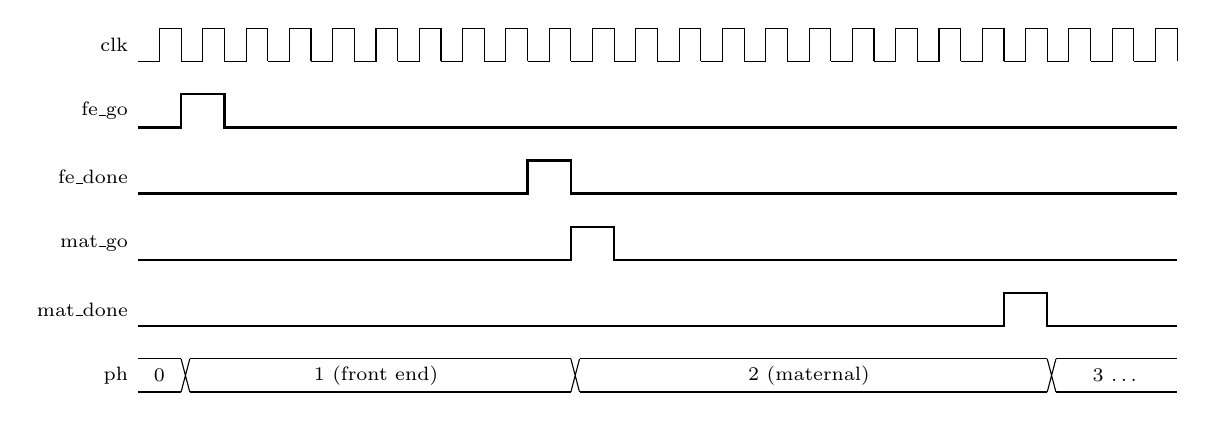
\begin{tikzpicture}[x=0.55cm,y=0.42cm]
\foreach \y/\n in {0/clk,-2/fe\_go,-4/fe\_done,-6/mat\_go,-8/mat\_done,-10/ph} \node[left,font=\scriptsize] at (0,\y+0.5) {\n};
\foreach \x in {0,...,23} \draw (\x,0) -- (\x+0.5,0) -- (\x+0.5,1) -- (\x+1,1) -- (\x+1,0);
\draw[thick] (0,-2) -- (1,-2) -- (1,-1) -- (2,-1) -- (2,-2) -- (24,-2);
\draw[thick] (0,-4) -- (9,-4) -- (9,-3) -- (10,-3) -- (10,-4) -- (24,-4);
\draw[thick] (0,-6) -- (10,-6) -- (10,-5) -- (11,-5) -- (11,-6) -- (24,-6);
\draw[thick] (0,-8) -- (20,-8) -- (20,-7) -- (21,-7) -- (21,-8) -- (24,-8);
\draw (0,-10) -- (1,-10) (0,-9) -- (1,-9); \draw (1,-10) -- (1.2,-9) (1,-9) -- (1.2,-10);
\draw (1.2,-10) -- (10,-10) (1.2,-9) -- (10,-9); \draw (10,-10) -- (10.2,-9) (10,-9) -- (10.2,-10);
\draw (10.2,-10) -- (21,-10) (10.2,-9) -- (21,-9); \draw (21,-10) -- (21.2,-9) (21,-9) -- (21.2,-10);
\draw (21.2,-10) -- (24,-10) (21.2,-9) -- (24,-9);
\node[font=\scriptsize] at (0.5,-9.5) {0}; \node[font=\scriptsize] at (5.5,-9.5) {1 (front end)}; \node[font=\scriptsize] at (15.5,-9.5) {2 (maternal)}; \node[font=\scriptsize] at (22.6,-9.5) {3 \dots};
\end{tikzpicture}
\caption{The go/done hand-shake of the sequencer (schematic). \mods{v6_core} pulses \mods{fe_go}, waits for \mods{fe_done}, then pulses \mods{mat_go}, and so on. The register \mods{ph} records which unit is active and steers the shared ports. A real sample from the simulation is in Fig.~\ref{fig:waveone}.}
\label{fig:handshake}
\end{figure}

\subsection{Timing: slack and WNS}\label{sec:timing}
Between two flip-flops there is a chain of logic and wires. A signal leaves the first flip-flop at a clock edge and must arrive at the second \emph{before} the next edge (minus a small set-up time). At 50\,MHz there are 20\,ns.
\[
\text{slack} = \text{time available (20 ns)} - \text{time the path needs}.
\]
Positive slack: the path is fast enough. Negative slack: at this clock the flip-flop might capture a half-finished, wrong value. The tool checks every path; the \term{worst negative slack} (\term{WNS}) is the slack of the slowest path (despite the name it is positive when timing is met). There is also a \emph{hold} check (data must not change too soon after the edge); its worst value is called WHS.

\begin{center}
\begin{tikzpicture}[x=0.6cm]
\draw[thick] (0,0) -- (20,0);
\foreach \x in {0,20} {\draw (\x,-0.2) -- (\x,0.2);}
\node[below,font=\scriptsize] at (0,-0.2) {edge 1 (0 ns)}; \node[below,font=\scriptsize] at (20,-0.2) {edge 2 (20 ns)};
\fill[tmblue!40] (0,0.3) rectangle (8.82,0.9); \node[font=\scriptsize] at (4.4,0.6) {logic 8.8 ns};
\fill[tmorange!50] (8.82,0.3) rectangle (19.79,0.9); \node[font=\scriptsize] at (14.3,0.6) {wires (routing) 11.0 ns};
\draw[<-] (19.9,1.0) -- (19.9,1.5) node[above,font=\scriptsize]{slack +0.048 ns};
\end{tikzpicture}
\end{center}
This is the real worst path of v7-DL (from \file{build/v7/timing.rpt}): 19.791\,ns of the 20-ns period, 29 logic levels, 44.6\% logic and 55.4\% wire delay. It meets timing with $+0.048$\,ns to spare.

\subsection{From Verilog to a running board}
\begin{enumerate}
  \item \term{Simulation} (we use \term{xsim}, the Vivado simulator): a program pretends to be the circuit and computes every signal, cycle by cycle. It is slow (minutes for seconds of recording), but you can see every internal signal. A \term{testbench} is Verilog that is \emph{not} hardware: it feeds inputs to your design and checks its outputs.
  \item \term{Synthesis}: Vivado translates the Verilog into LUTs, flip-flops, BRAMs and DSPs (a ``netlist'').
  \item \term{Implementation}: \emph{placement} (where on the chip each piece sits), \emph{routing} (which wires connect them), then \emph{static timing analysis} (the slack of every path).
  \item \term{Bitstream} generation: the configuration file (e.g.\ \file{build/v7/v7.bit}).
  \item \term{Programming}: load the bitstream over JTAG (the USB cable) into the FPGA.
  \item \textbf{Board run}: real hardware, real UART, real PC.
\end{enumerate}
\textbf{Out-of-context (OOC) synthesis} means synthesising one module on its own, without the rest of the design. It is quick and tells you how big that module is by itself. The 13.2k and 8.4k LUT figures of \mods{v7_la} are stand-alone figures of this kind; inside the routed full design Vivado reports 7,297 LUTs for it, because optimisation across module boundaries changes the count.

\begin{lesson}[Simulation vs timing analysis vs board]
Simulation proves that the \emph{logic} is right (the same bytes as the C model). Static timing analysis proves that the \emph{real chip} is fast enough for that logic at 50\,MHz. The board run proves both together on real hardware, with the real UART and PC. You need all three.
\end{lesson}

\subsection{Fixed-point integer arithmetic}\label{sec:fixed}
Floating-point numbers (like \mods{float} in C) are expensive in FPGA logic, and their rounding depends on the order of operations. We use \term{fixed point}: a real number is stored as an integer with an agreed number of \emph{fraction bits}. In format \term{Q$n$}, the stored integer $I$ means $I / 2^n$.
\begin{itemize}
  \item Q8: $256 = 1.0$, $128 = 0.5$. Our filter data.
  \item Q14: $16384 = 1.0$. Spatial weights and maternal projections (16-bit, so a range of about $\pm 2$).
  \item Q22 in 24 bits (``s24''): $4{,}194{,}304 = 1.0$. Template basis entries ($|v| \le 1$).
  \item Q28: $268{,}435{,}456 = 1.0$. Filter coefficients. Example: the first low-pass coefficient \mods{22192263} means $22192263/2^{28} \approx 0.0827$.
\end{itemize}

\textbf{Multiplying.} Q$a$ times Q$b$ gives Q$(a+b)$. To get back to fewer fraction bits you shift right. Example: data Q8 times coefficient Q28 = Q36; shift right by 28 to get Q8 again. Intermediate products are kept in \textbf{64-bit accumulators} so that nothing overflows.

\textbf{Rounding.} A plain right shift rounds down. We round to nearest: add half of the last kept bit, then shift:
\[
\text{rnd}(a, s) = (a + 2^{s-1}) \gg s .
\]
In Verilog this is e.g.\ \mods{(acc + 64'sd8192) >>> 14} (round away 14 fraction bits).

\textbf{Saturation.} If a value is too big for its bits, clip it to the largest or smallest value instead of letting it wrap around (wrapping turns a big positive number into a big negative one). \mods{sat16} clips to $[-32768, 32767]$.

\textbf{Overflow check.} The C model checks every value against the width it has in hardware (\mods{chk(v, bits)} sets \mods{fm_overflow}). The report: no value left its declared width on any record.

\textbf{Exact comparisons.} ``Accept a beat if $e > 0.25 \times \text{median}$'' becomes the integer test $4e > m$ (or $8e > a + b$ when the median is the mean of the two middle values). No rounding doubt is left, so C and Verilog always agree.

\begin{keyfact}[Number formats of v6 (C model = RTL)]
Raw input int16; filter data Q8 in int32; SOS coefficients Q28; products and accumulators 64-bit; $\mathbf{z}$ and $\mathbf{x}_f$ stored as int16; envelopes as 16-bit monotonic codes with 8 significant bits; spatial weights and maternal projections Q14; template basis s24 Q22; tracker autocorrelation 15-bit block floating point; v7 quality $\log_2$ in Q8.
\end{keyfact}

\subsubsection*{The envelope code: a tiny floating point}
Envelope values (sums of squares) can be anywhere from 0 to almost $2^{64}$. Storing 64 bits for each of $16 \times 2048$ envelope samples would waste memory. So \mods{enc_e} (in \file{proto.h}, with a copy in \mods{v6_trk}) stores a 16-bit code: values below 256 as themselves, larger values as an exponent plus the top 8 significant bits (rounded). Example: $x = 1000$. Its leading one is bit 9, so we shift right by 2: mantissa $m = 250$, code $= (2+1)\cdot128 + (250 - 128) = 506$. Decoding gives $(128 + 122) \ll 2 = 1000$. The code is \emph{monotonic}: a larger value never gets a smaller code, so ``which envelope is bigger?'' can be decided on the codes directly. The largest possible code (for $x$ near $2^{64}$) is $57\cdot128 + 127 = 7{,}423 < 2^{13} = 8192$, so 13 bits are always enough. That fact made the BRAM sharing possible (Section~\ref{sec:bram}).

\textbf{Block floating point.} For the tracker autocorrelation, 1,000 envelope values are decoded and all shifted right by the \emph{same} amount so that the largest fits in 15 bits. The whole block shares one exponent, so the products are small and the result is exact and repeatable.

\subsection{The algorithm, just enough to read the hardware}
\subsubsection*{Filters: the biquad (SOS)}
A digital filter computes each output from the current input and a few remembered values. Our filters are chains of \term{second-order sections} (SOS, ``biquads''). One section in the ``direct form II transposed'' (DF2T) used by \mods{v6_sos}:
\begin{align*}
y &= \text{rnd}(b_0 x + z_1,\ 28)\\
z_1 &\leftarrow b_1 x - a_1 y + z_2\\
z_2 &\leftarrow b_2 x - a_2 y
\end{align*}
$b_0, b_1, b_2, a_1, a_2$ are the five Q28 coefficients; $z_1, z_2$ are the two 64-bit state values the section remembers between samples. The output of one section is the input of the next. There are three coefficient sets: low-pass (2 sections), maternal band (2 sections) and track band-pass (4 sections). The front-end high-pass is a one-pole filter: a running baseline $B \leftarrow B + ((x\ll16) - B) \gg 6$ and output $h = (x \ll 8) - \text{rnd}(B, 8)$ (the report gives a cut-off of about 0.63\,Hz).

\subsubsection*{Maternal PCA and detectors}
Four leads give four numbers per sample. The $4\times4$ \term{covariance} (average products of pairs of leads) describes how the leads move together. \term{PCA} finds the directions (weight vectors) with the most power; on the belly that is mostly the mother. Each projection $y_k = \sum_l V_{kl}\, y_{m,l}$ is squared, smoothed by a \term{moving-window integrator} (MWI: the running sum of the last 38 values) and fed to an \term{adaptive-threshold detector}. The detector learns a ``peak level'' and a ``noise level'' over a 512-sample warm-up, puts the threshold at $(\text{peak} + 3\,\text{noise})/4$, finds local maxima above it, blocks a second detection for a \emph{refractory} time (75 samples), and places the exact peak at the largest $|y|$ in the last 30 samples.

\subsubsection*{Template cancellation as a projection}
For each maternal beat the segment $\mathbf{s}$ (150 samples of one lead) is approximated by a combination of up to three basis vectors (mean and two principal components of the last 20 beats). If the PC makes the basis \emph{orthonormal} (unit length, at right angles to each other), the best least-squares fit is simply the \term{projection}
\[
\hat{\mathbf{s}} = \mathbf{Q}\mathbf{Q}^T\mathbf{s}, \qquad c_j = \langle \mathbf{q}_j, \mathbf{s} \rangle,\quad \hat{\mathbf{s}} = \textstyle\sum_j c_j \mathbf{q}_j ,
\]
which is only dot products and multiply-adds: no matrix inversion in hardware. The fit is subtracted with \emph{tapered} edges: the first and last 8 samples of the fit are scaled down linearly (weights $0, \tfrac17, \dots, 1$ in Q15), so no step appears at the window borders. v5 solved the least-squares problem with a Gauss--Jordan solve; the projection onto a PC-orthonormalised basis spans the same space, so the fit is mathematically the same.

\subsubsection*{GEVD spatial filters, envelopes, trackers}
A \term{GEVD} filter is a weight vector $\mathbf{w}$ that maximises (power around the fetal beats) / (total power). The PC computes 16 of them; in the FPGA each is just $y = \sum_l w_l x_l$ (4 multiply-adds). The track signal is band-passed, squared and summed over 30 samples: the \term{energy envelope}, in which beats become bumps. A \term{tracker} first estimates the beat period $R$ by \term{autocorrelation} (how similar the envelope is to a copy of itself shifted by a lag; the best lag between 75 and 166 samples, i.e.\ 200 to 90\,bpm, is the period). It then looks for each next beat at 70--130\% of $R$ after the last one, accepts the biggest peak there if it is above a quarter of the median of recent beat sizes, updates $R$ as the median of the last five intervals, and restarts after four misses in a row.

\subsubsection*{Look-ahead and Viterbi (v7-DL)}
For every 2.5-s \emph{segment}, each of the 16 tracks gets a quality score computed over a window that includes 7.5\,s of the future (the unit simply waits for it). A \term{Viterbi} step keeps, for each track, the best total score of any sequence of track choices that ends in that track, where changing track costs a penalty. The chosen track's beats are then cleaned (fill one missed beat, drop a beat that splits an interval), and each final beat gets a centred FHR (median of 5 intervals around it).

% =====================================================================
\section{Your part, from the start: what was tried, why, and what happened}
% =====================================================================
This section tells the story in time order. Each ``What we tried'' box gives the idea, the reason, the measured result and the decision. Dates come from the git history and the logs.

\begin{center}
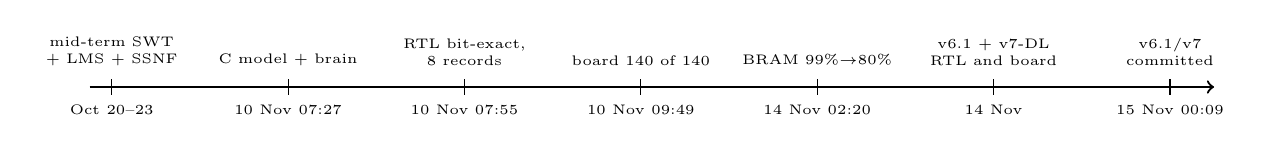
\begin{tikzpicture}[x=0.56cm,y=0.5cm]
\draw[thick,->] (-0.5,0) -- (25,0);
\foreach \x/\d/\t in {0/{Oct 20--23}/{mid-term SWT + LMS + SSNF},4/{10 Nov 07:27}/{C model + brain},8/{10 Nov 07:55}/{RTL bit-exact, 8 records},12/{10 Nov 09:49}/{board 140 of 140},16/{14 Nov 02:20}/{BRAM 99\%$\to$80\%},20/{14 Nov}/{v6.1 + v7-DL RTL and board},24/{15 Nov 00:09}/{v6.1/v7 committed}}
  {\draw (\x,-0.2) -- (\x,0.2); \node[above,font=\tiny,align=center,text width=1.9cm] at (\x,0.3) {\t}; \node[below,font=\tiny] at (\x,-0.2) {\d};}
\end{tikzpicture}
\end{center}

\subsection{Mid-term (October): the SWT + LMS + SSNF wavelet hybrid}
At mid-term each member implemented one or more extraction methods, and all were compared on the same five FECGSYNDB test cases (TC1--TC5, subject 1: 12, 6 and 0\,dB baseline, fetal movement, ectopic beats). Your method (\file{code/src/methods/swt_lms_ssnf.py}) adapts Karvounis \emph{et al.}\ (2013) to a single abdominal lead.

\begin{simple}[What the method does, step by step]
\begin{enumerate}
  \item \textbf{Find maternal R peaks} on the mixture (peaks above 45\% of a robust amplitude scale, at least 400\,ms apart).
  \item \textbf{Build a maternal reference.} The original paper uses a real chest (thoracic) lead as the reference for the adaptive filter. FECGSYNDB has no separate thoracic reference file in our set-up, so the method \emph{synthesises} a reference: the median maternal beat ($\pm 300$\,ms around each R peak) placed at every detected peak.
  \item \textbf{Stationary Wavelet Transform (SWT).} Split both the mixture and the reference into frequency bands (``subbands'') with a 4-level SWT using the \texttt{sym4} wavelet. ``Stationary'' means no down-sampling, so every subband keeps the full time resolution (shift-invariant).
  \item \textbf{LMS in every subband.} A 32-tap normalised LMS adaptive filter (step size $\mu = 0.05$) predicts the maternal part of each subband from the reference subband and subtracts it.
  \item \textbf{SSNF.} Inter-scale soft thresholding: wavelet coefficients below $3\times$ a robust (MAD-based) noise level are shrunk towards zero, to suppress residual maternal energy and muscle noise while keeping the sharp fetal QRS.
  \item \textbf{Inverse SWT} gives the estimated fetal ECG; the common mid-term detector finds the beats.
\end{enumerate}
\end{simple}

\begin{tried}[Mid-term method: SWT + LMS + SSNF on one lead]
\what{Wavelet subband decomposition + per-subband LMS cancellation against a synthetic maternal reference + soft thresholding, on lead 27 of FECGSYNDB.}
\why{Adaptive noise cancelling (Widrow 1975) is the classic way to remove an interfering signal when you have a reference for it; wavelets separate the sharp QRS from slow waves.}
\result{Very poor: F1 15.06\% on TC1 (12\,dB), 17.56\% (TC2), 19.15\% (TC3), 18.50\% (TC4), 14.57\% (TC5); mean 16.97\%, FHR MAE 46.92\,bpm. It was also slow (about 1.8\,s per 5-s window) and was rated ``High DSP ($>$100\% on XC7S50)'' in the mid-term sizing. The 4-lead spatial PCA reached 100\% on TC1--TC3.}
\decision{Dropped. The report explains the failure: a single abdominal mixture has no pure maternal reference, so the LMS filter actively cancels fetal complexes too. In the final report the method is replication R4 (``qualitative only: failure mechanism consistent'') and correction C-12 fixed its description to ``SWT + LMS + SSNF''.}
\end{tried}

\begin{figure}[H]
\centering
\includegraphics[width=0.82\linewidth]{TC3_swt_lms_ssnf.png}
\caption{Your mid-term method on TC3 (0\,dB): mixture (top), clean fetal reference used only for scoring (middle), extracted signal with reference peaks (green) and detected peaks (red, bottom). Detections often miss the true beats.}
\end{figure}

\begin{lesson}
The mid-term taught the whole team that single-lead temporal methods fail when maternal and fetal beats overlap, and pushed us towards multi-lead (spatial) processing. Your own method was a negative result, but an honest one: say so in the viva. In the report's mid-term tables it appears as ``SWT-LMS Wavelet Filter''; do not confuse it with the ``Wavelet-Threshold Hybrid'' row, which is Vivek's method.
\end{lesson}

\subsection{Late October to 9 November: what happened before your final part}
After the mid-term the team changed the rules (strictly causal, no labels, real recordings, held-out test). The mid-term design fell to 16.7\% on held-out CinC. Anshu designed a new algorithm (v3, v4 in Python), and on the night of 9--10 November Vivek ported it to C on a \term{MicroBlaze} soft processor inside the FPGA (v5): 65.8\% on CinC test, bit-exact with the PC build of the same C code on 140 records.

\begin{tried}[v5: the whole algorithm as C on a MicroBlaze (Vivek's version, the starting point of your part)]
\what{A processor built from FPGA logic (with a floating-point unit, 73.7\,MHz) runs the C program; the PC only streams the recording.}
\why{Writing RTL for GEVD, template fitting and 12 trackers in one night was not feasible.}
\result{It worked: 3,340 LUTs, 5 DSP, 72 of 75 BRAM tiles; about 47k cycles per sample, $5.4\times$ real time after a $3.5\times$ speed-up. But (1) the hardware was a processor \emph{we did not design}, and (2) the memory was full: 254.6 of 256\,KB local memory and 30.4 of 32\,KB AXI memory (\file{report/night_20261109/RESULTS.md}).}
\decision{For the final design, move every sample-rate operation into our own RTL (``Why v6'' in the report). That is your part.}
\end{tried}

\subsection{10 November: the hardware/PC split by rate}
The goal written in the v6 log: \emph{``redistribute work between the FPGA and the PC so the FPGA part is hand-written RTL (no soft processor), giving the PC the minimum work needed to keep v5-level accuracy.''}

\begin{tried}[Split the v5 algorithm by rate]
\what{Everything that runs 250 times per second goes into RTL. Only decisions that happen between once per recording and about once per maternal beat (1--1.5\,Hz) go to a PC ``brain'' (\file{model/brain.c}).}
\why{Sample-rate work is regular and simple (multiply-adds, comparisons) and must be fast: ideal for hardware. The slow decisions need eigen-decompositions with square roots, divisions and refinement loops in floating point, plus a lot of memory: expensive in RTL, but needed only a few times per second.}
\result{Five decisions remain on the PC (Table~\ref{tab:five}). The PC receives only messages computed by the FPGA, never the raw recording. The FPGA stalls on each request until the answer arrives, so the result never depends on the PC's speed.}
\decision{Adopted; it is the architecture of v6, v6.1 and v7-DL (Fig.~\ref{fig:arch}).}
\end{tried}

\begin{table}[H]
\centering\small
\begin{tabularx}{\linewidth}{@{}>{\raggedright\arraybackslash}p{2.4cm}>{\raggedright\arraybackslash}p{2.5cm}>{\raggedright\arraybackslash}X>{\raggedright\arraybackslash}X@{}}
\toprule
\textbf{Decision} & \textbf{How often} & \textbf{FPGA sends} & \textbf{PC returns} \\
\midrule
Maternal PCA & once, at 10\,s & $4\times4$ covariance (COV) & 4 projection vectors, Q14 (RSP\_V) \\
Maternal train & every 5\,s & detector peak events (MDET), REQ\_MK & train index (RSP\_MK) \\
Template basis & per maternal beat & aligned $150\times4$ beat segment (SEG) & orthonormal basis, $\le 3\times150$ per lead, s24 Q22 (RSP\_BASIS) \\
GEVD calibration & at 15\,s (v6.1: + every 30\,s) & 12\,s of $\mathbf{z}$ and $\mathbf{x}_f$, int16 (CALDATA), REQ\_CAL & 16 weight vectors Q14 + track flags (RSP\_CAL) \\
Track selection & every 2.5\,s & beats, snapshots, envelope medians (BEAT, FEAT, BMED), REQ\_SEL & track index (RSP\_SEL) \\
\bottomrule
\end{tabularx}
\caption{The five PC decisions (report, Tab.\ ``The five decisions left to the PC''; \file{model/proto.h}).}
\label{tab:five}
\end{table}

\begin{figure}[H]
\centering
\includegraphics[width=\linewidth]{fin_v6_architecture.png}
\caption{Architecture of v6 (report figure). Everything at the sample rate is hand-written Verilog. The FPGA sends five kinds of requests and stalls until the answer arrives. v6.1 and v7-DL add units to this.}
\label{fig:arch}
\end{figure}

\subsubsection*{Why the PC stays in the loop (report Sec.\ ``Why the PC Stays in the Loop'')}
This is a likely viva attack, so know the four measured reasons.

\begin{table}[H]
\centering\small
\begin{tabularx}{\linewidth}{@{}llrX@{}}
\toprule
\textbf{Decision} & \textbf{Rate} & \textbf{Traffic} & \textbf{On the FPGA it would need} \\
\midrule
Template basis & per maternal beat & 59.1\% & 20-beat history (24\,KB, about 6 BRAM tiles) and a $20\times20$ subspace iteration with square roots and divisions \\
Track selection & every 2.5\,s & 28.7\% & floating-point log-quality of 16 tracks; in v7-DL the final beats already come from the on-chip look-ahead unit \\
GEVD calibration & 15\,s, then every 30\,s & 11.6\% & 48-KB buffer of $\mathbf{z}$ and $\mathbf{x}_f$ (about 12 tiles) and a generalised $4\times4$ eigen-solver with refinement \\
Maternal train / PCA & every 5\,s / once & 0.6\% & train statistics / one $4\times4$ eigen-decomposition \\
\bottomrule
\end{tabularx}
\caption{Share of the link traffic of v7-DL per decision (C model on ADFECGDB r01, 120\,s; \file{report/final_report/tables/pc_link_traffic.csv}).}
\label{tab:traffic}
\end{table}
\begin{enumerate}
  \item \textbf{Memory.} The brain's C implementation keeps about 200\,KB of state (beat history, calibration buffers, track features), as much as about 50 of the 75 BRAM tiles. v7-DL leaves only 4 tiles free. A soft processor running the brain would need the same memory plus its program; v5 showed a MicroBlaze running the whole algorithm fills 72 of 75 tiles.
  \item \textbf{Arithmetic.} Basis and GEVD need eigen-decompositions with square roots, divisions and refinement loops in floating point; each would need its own iterative solver in RTL, to run a few times per second at most, on a chip already 82\% full of LUTs.
  \item \textbf{Accuracy.} The PC versions give the reported accuracy. The cheaper on-chip alternative that was measured, a running (EMA) template instead of the basis, lost 1.1 points on CinC dev.
  \item \textbf{No real-time cost.} With the PC in the loop the v7-DL board runs 3.4--5.6$\times$ faster than real time (mean $4.35\times$; v6: 3.7--9.4$\times$, mean $4.81\times$), and the RTL alone about $135\times$.
\end{enumerate}
The link is lightly loaded: v7-DL uses 7.8\,KB/s up and 9.2\,KB/s down, 8--10\% of the 92\,KB/s that 921,600 baud carries in each direction. For v6 the log gives about 9.4\,KB/s down (samples 2\,KB/s, template bases 7.3\,KB/s) and 7.2\,KB/s up (features 4.6, segments 1.6, rest about 1\,KB/s), so the link would allow up to roughly $10\times$ real time.

\begin{keyfact}[The path to a stand-alone device (report)]
On an FPGA with a hard processor (e.g.\ a Zynq SoC) the RTL could stay largely as it is and \file{brain.c} would run on the processor instead of the laptop. On the Spartan-7 itself the most direct step: in v7-DL the PC's selection only drives the \emph{live} output, so taking the live track from the scores \mods{v7_la} already computes would remove 28.7\% of the traffic and one decision. The template basis could move on chip only by freeing BRAM, or as a running template at the measured cost of 1.1 points. Neither step has been implemented.
\end{keyfact}

\subsection{10 November: the bit-accurate C model first}
\begin{tried}[Write an integer C model of exactly what the FPGA will compute, before any Verilog]
\what{\file{model/fpga_model.c} (661 lines): every sample-rate operation in integers, in the same order as the hardware. \file{brain.c} is the PC brain; \file{sim_main.c} connects the two through the \emph{real} message protocol, with the board host's lock-step framing (64-sample frames, each answered by DONE). The model \emph{stalls} on a request until the brain's answer is there (\mods{wait_rsp}), exactly like the hardware.}
\why{(1) Accuracy can be measured quickly on all records with the model, long before the hardware exists. (2) The model writes a ``golden'' byte stream that the RTL must reproduce byte for byte, so any RTL bug shows up as the first differing byte. (3) It forces every rounding, width and order decision to be made once, explicitly.}
\result{The model matched v5's accuracy (all differences within $\pm0.8$ points), and no value left its declared hardware width on any record (overflow checks). Numbers below.}
\decision{The C model became the \emph{specification}. Rule for every later change: C model first $\to$ RTL $\to$ \mods{sim/regress.sh} $\to$ build $\to$ board (\file{PLANNED_CHANGES.md}).}
\end{tried}

\begin{table}[H]
\centering\small
\begin{tabular}{@{}lrr@{}}
\toprule
\textbf{Set} & \textbf{v5 (board)} & \textbf{v6 C system model} \\
\midrule
FECGSYNDB subset (60) & 91.92 & 91.83 \\
FECGSYNDB all 1,248 & 91.46 (PC model) & 91.44 \\
CinC dev (38) & 75.26 & 76.04 \\
ADFECGDB (5) & 93.44 & 92.73 \\
\bottomrule
\end{tabular}
\caption{Mean F1 (\%) of the v6 C system model against v5 (\file{report/rtl_pc_split/LOG.md}).}
\end{table}

What changed against v5 to make the model hardware-friendly (all listed in the report):
\begin{itemize}
  \item float filters $\to$ Q8 data, Q28 coefficients, 64-bit accumulators;
  \item v5's bf16 envelopes $\to$ 16-bit monotonic codes with 8 significant bits (the same precision);
  \item tracker autocorrelation $\to$ 15-bit block floating point;
  \item every threshold comparison $\to$ an exact integer test ($0.25\times$median $\to$ $4e > m$ or $8e > a+b$);
  \item template least-squares solve $\to$ projection $\mathbf{Q}\mathbf{Q}^T\mathbf{s}$ onto the PC-orthonormalised basis (same span, same fit).
\end{itemize}

\textbf{Build switches.} The same files build three versions: no define = frozen v6 (matches \file{build/v6.bit}); \mods{-DV61} = v6.1; \mods{-DV7} = v7-DL (switches on \mods{V61} too). The Verilog uses the same defines. The C build uses fixed flags (\mods{-msse2 -mfpmath=sse -ffp-contract=off}) because other flags can change the floating-point results of the brain and break bit-exactness.

\subsection{10 November: the hand-written Verilog datapath}
\begin{tried}[One sequential datapath, in the order of the C model]
\what{About 1,800 lines of Verilog in eleven files (report): UART, frame parser and FIFOs, a time-multiplexed SOS biquad engine, moving-window integrators, adaptive-threshold detectors, the front end, the maternal block, the canceller and the 16-track block. A sequencer in \mods{v6_core} runs, for each sample, front end $\to$ maternal $\to$ canceller $\to$ calibration data $\to$ tracks, exactly the order of \mods{fm_push} in the C model.}
\why{Processing one sample at a time in the model's order makes the RTL easy to compare with the model: the same values are computed in the same order, so the output bytes come out in the same order. Time-multiplexed engines keep the area small because cycles are plentiful (200,000 per sample).}
\result{Bit-exact with the C model on 8 records in xsim the same morning (07:55), see below.}
\decision{This is the final architecture; v6.1 and v7-DL only add to it.}
\end{tried}

The module hierarchy (details in Section~\ref{sec:walk}):
\begin{center}
\begin{tikzpicture}[every node/.style={font=\small},level distance=0.75cm]
\node[blk,text width=11cm] (top) {\mods{v6_top}: 100$\to$50\,MHz PLL, reset, UART RX/TX (\mods{v6_uart}), LEDs; in v7: \mods{v7_disp}};
\node[blk,text width=11cm,below=0.35cm of top] (core) {\mods{v6_core}: sequencer, $\mathbf{x}_f$ and $\mathbf{z}$ rings ($4096\times64$), shared memory \mods{umem} ($32\text{K}\times13$), port multiplexers};
\node[blk,below left=0.45cm and -2.6cm of core,text width=2.3cm] (l) {\mods{v6_link}\\frames, FIFOs};
\node[blk,right=0.15cm of l,text width=1.9cm] (f) {\mods{v6_fe}\\uses \mods{v6_sos}};
\node[blk,right=0.15cm of f,text width=2.4cm] (m) {\mods{v6_mat}\\ mwi, det};
\node[blk,right=0.15cm of m,text width=1.6cm] (c) {\mods{v6_canc}};
\node[blk,right=0.15cm of c,text width=2.6cm] (t) {\mods{v6_trk}\\sos, mwi, det};
\node[blk,below=0.3cm of m,text width=5cm,fill=tmgreenl] (la) {\mods{v7_la} (v7-DL only): look-ahead};
\draw (top) -- (core);
\foreach \n in {l,f,m,c,t} \draw (core.south) -- (\n.north);
\draw[dashed] (core.south) -- (la.north);
\end{tikzpicture}
\end{center}

\subsection{10 November: testbenches and the regression}\label{sec:tb}
\begin{tried}[Verify the RTL against the C model, unit by unit and then as a whole system]
\what{\textbf{Unit tests} (xsim): \file{sim/tb_sos.v} drives the SOS engine with 3,000 inputs through each of the three filter sets (9,000 outputs) and compares with vectors from \file{gen_sos.c}; \file{sim/tb_det.v} drives two MWI + detector instances (the maternal and the track parameter sets) with 20,000 samples each and compares with \file{gen_det.c}. \textbf{System test} \file{sim/tb_core.v}: the testbench plays the board host. It sends the recording in 64-sample SAMPLES frames (waiting for DONE after each), replays the PC brain's answers when the frame that triggers them has arrived, and compares \emph{every uplink byte} with the golden stream of the C model.}
\why{Unit tests find arithmetic mistakes early in a small engine; the system test checks the complete behaviour, including every message, every request and the timing-independence of the protocol.}
\result{Units: 0 errors. System: 8 records, 0 byte errors (Table~\ref{tab:xsim6}).}
\decision{\mods{sim/regress.sh} became the gate for every change (also used for v6.1 and v7-DL).}
\end{tried}

\begin{table}[H]
\centering\small
\begin{tabular}{@{}lrrrr@{}}
\toprule
\textbf{Record} & \textbf{Length} & \textbf{Uplink bytes} & \textbf{Frames} & \textbf{Byte errors} \\
\midrule
CinC a01 & 60\,s & 406,454 & 6,580 & 0 \\
CinC a07 & 60\,s & 409,771 & 6,473 & 0 \\
CinC a29 & 60\,s & 394,992 & 6,104 & 0 \\
CinC a65 & 60\,s & 427,056 & 6,114 & 0 \\
CinC a71 & 60\,s & 417,980 & 6,707 & 0 \\
ADFECGDB r01 & 120\,s & 838,652 & 13,532 & 0 \\
FECGSYNDB sub01 l1 c0 & 120\,s & 976,056 & 14,660 & 0 \\
FECGSYNDB sub01 l5 c1 & 120\,s & 1,047,441 & 15,669 & 0 \\
\bottomrule
\end{tabular}
\caption{v6 system testbench results (\file{report/rtl_pc_split/LOG.md}).}
\label{tab:xsim6}
\end{table}

\textbf{Bugs found.} The tests found a wrong SEG frame length: 604 instead of 1,204 bytes. A SEG payload is a 4-byte time stamp plus $150 \times 4$ samples of 2 bytes each $= 4 + 1200 = 1204$; the wrong value $4 + 600$ counted samples instead of bytes. Fixes made during code review, before simulation: the signedness of the detector constants, a 4-bit loop index that could not reach 16, and the byte packing of the track id.

\begin{simple}[How the regression works (\file{sim/regress.sh})]
For each recording file (\file{.i16}: raw int16, 4 leads):
\begin{enumerate}
  \item \mods{V6_DUMP=G ../model/v6_sim.exe rec.i16} runs the C system model and writes two files: \file{G_up.hex} (every uplink byte, one per line) and \file{G_script.txt} (the host's actions in order: ``\mods{S}'' send this SAMPLES frame; ``\mods{R i ...}'' send this PC answer once uplink frame $i$ has arrived; ``\mods{F}'' send FLUSH (v7); ``\mods{E}'' end).
  \item \file{run_tb.sh} compiles the RTL and \file{tb_core.v} with \mods{xvlog} (with \mods{DEFS="-d V61 -d V7"} for v7), elaborates with \mods{xelab} and runs \mods{xsim}.
  \item The testbench prints \mods{MISMATCH} lines (stops after 20) and a final \mods{RESULT: n uplink bytes, m frames, e byte errors}.
\end{enumerate}
In the testbench the PC answers instantly and each byte takes two clock cycles, so simulated time is pure FPGA processing time.
\end{simple}

\subsection{10 November: implementation}\label{sec:impl}
\begin{tried}[First Vivado build of v6]
\what{\file{build_v6.tcl}: XC7S50, PLL 100$\to$50\,MHz, UART 921,600 baud.}
\why{To get a bitstream and check resources and timing.}
\result{Two fixes were needed: (1) the $\mathbf{z}$ ring was written from two places (front end and canceller), so it could not map to block RAM and the tools built it from LUT RAM (``distributed-RAM overuse''); it was merged to a \emph{single write port} with a multiplexer (\mods{z_we = fe_we | ca_zwe}) so it maps to block RAM. (2) A sorting-network loop failed synthesis (error 8-3380) and was rewritten. The first build then used 19.0k LUTs (3.4k as LUT RAM, 58\%), 10.1k FFs, 33 DSP, \textbf{74.5 of 75 BRAM tiles (99\%)}, worst slack $+0.49$\,ns at 50\,MHz.}
\decision{Timing met; the near-full block RAM was noted and fixed later (Section~\ref{sec:bram}).}
\end{tried}

\subsection{10 November: first board run, 140/140 bit-exact}
\file{uart_host/run_v6_board_eval.py} (Vivek's script) streams each record, runs the brain as a pipe, scores the beats and compares the board's \emph{complete} uplink byte stream with the C model.

\begin{table}[H]
\centering\small
\begin{tabular}{@{}lrrrrrrr@{}}
\toprule
\textbf{Set} & \textbf{Rec.} & \textbf{F1} & \textbf{Se} & \textbf{PPV} & \textbf{FHR MAE} & \textbf{Bit-exact} & \textbf{Speed} \\
\midrule
FECGSYNDB subset & 60 & 91.83 & 90.67 & 93.65 & 5.24 & 60/60 & 4.3$\times$ \\
ADFECGDB & 5 & 92.73 & 91.16 & 94.37 & 2.03 & 5/5 & 4.6$\times$ \\
CinC dev & 38 & 76.04 & 74.45 & 77.98 & 12.52 & 38/38 & 4.8$\times$ \\
\textbf{CinC test (held out)} & 37 & \textbf{65.48} & 64.39 & 67.00 & 18.37 & 37/37 & 5.1$\times$ \\
\bottomrule
\end{tabular}
\caption{v6 on the board (report, Tab.\ ``Results of v6 measured on the Spartan-7 board''). Speed = record length / streaming time, including UART and PC.}
\end{table}
The board equals the model on all 140 records, so the board F1 equals the model F1 on every set. Accuracy matches v5 within $\pm 0.8$ points, now without a soft processor.

\begin{figure}[H]
\centering
\includegraphics[width=0.72\linewidth]{fin_board_speed.png}
\caption{Board speed per record of v6 (report figure): every record 3.7--9.4$\times$ faster than real time (mean of per-record ratios $4.81\times$). On CinC a01 via the web page the median time per 64-sample frame was 34\,ms, with a one-off peak of 0.58\,s during calibration.}
\end{figure}

\subsection{14 November: measurements inside the RTL (waveforms)}
To show what happens inside the hardware, the unchanged system testbench was run on the first 30\,s of CinC a01 through a wrapper (\file{sim/wave/tb_wave.v}) that brings internal signals to the top, and dumped to a VCD file. The run is itself a test: all 164,447 output bytes (2,721 frames) matched the model and all 21 beats were identical.

\begin{figure}[H]
\centering
\includegraphics[width=\linewidth]{wave_overview.png}
\caption{The whole 30-s simulation (210.6\,ms of simulated time). First 10\,s fast (only storing), then the PCA request and the replay of 2,500 samples (flat \mods{sample_T}, rising \mods{mat_npeaks}), the GEVD request at 15\,s (\mods{calibrated}), the one-time tracker start at about 85--107\,ms, then OUT frames.}
\end{figure}

\begin{figure}[H]
\centering
\includegraphics[width=0.78\linewidth]{wave_one_sample.png}
\caption{One sample after calibration (T\,=\,6,100): \mods{fe_go}/\mods{fe_done}, \mods{mat_go}/\mods{mat_done}, \mods{ca_go}/\mods{ca_done} (no maternal beat, finishes at once), \mods{tk_go}/\mods{tk_done}; FEAT and BEAT frames leave meanwhile. 2,348 cycles = 47\,$\mu$s.}
\label{fig:waveone}
\end{figure}

\begin{figure}[H]
\centering
\begin{minipage}{0.49\linewidth}\includegraphics[width=\linewidth]{wave_pca_request.png}\end{minipage}\hfill
\begin{minipage}{0.49\linewidth}\includegraphics[width=\linewidth]{wave_cycles_per_sample.png}\end{minipage}
\caption{Left: a request to the PC (maternal PCA at T\,=\,2,499): COV goes out (\mods{tx_valid}), the FPGA waits, the answer arrives (\mods{rx_valid}), \mods{pca_answer} pulses, processing continues. Right: cycles per sample: median 301 before 10\,s, about 470 during calibration, 1,485 once all 16 tracks run; one peak of 1.12 million cycles (22\,ms) at the tracker start, absorbed by the 512-sample input FIFO.}
\end{figure}

\begin{keyfact}[Speed numbers and their two definitions]
\begin{itemize}
  \item Budget: $50\,\text{MHz} / 250\,\text{Hz} = 200{,}000$ cycles per sample.
  \item After calibration: median 1,485 cycles = 30\,$\mu$s per sample $\Rightarrow 200{,}000/1{,}485 \approx 135\times$ real time (the report's figure).
  \item Whole 30-s run: 210.6\,ms simulated $\Rightarrow \approx 142\times$ real time (about 7\,ms of FPGA time per second of signal).
  \item Board (v6): $4.81\times$ on average, because every sample and every PC request crosses the 921,600-baud UART and waits for the PC. The logic is not the bottleneck.
\end{itemize}
Older notes say ``about $140\times$''; the report corrected this (C-13, C-47) to $135\times$ (median) and $142\times$ (whole run). Use the report's numbers.
\end{keyfact}

\textbf{Why the 1.12-million-cycle peak?} When all 12 trackers start, each computes an autocorrelation over 1,000 envelope samples for 92 lags (75 to 166): roughly $12 \times 92 \times 1000 \approx 1.1$ million multiply-adds at one per cycle. It happens once; the input FIFO (512 samples = 2\,s of signal) holds the samples that arrive meanwhile.

\begin{figure}[H]
\centering
\includegraphics[width=0.95\linewidth]{wave_cancellation.png}
\caption{Maternal cancellation in the RTL, reconstructed from the simulated memory writes: lead 1 before (top) and after cancellation (middle), and the beats from the RTL and the C model (bottom): identical.}
\end{figure}

\textbf{Power.} Vivado's power analysis of the routed v6 design (default switching activity, confidence ``medium''): 0.374\,W on-chip, of which 0.299\,W dynamic (PLL 0.097, signals 0.065, logic 0.058, block RAM 0.050, DSP 0.015\,W) and 0.075\,W static, junction temperature 26.8\,\textdegree C. It is an estimate; the board was not measured.

\subsection{13--14 November: the block RAM reduction}\label{sec:bram}
The first build used 74.5 of 75 BRAM tiles. That left no room for anything new (and v6.1 and v7 were coming). \file{PLANNED_CHANGES.md} lists the tiles per memory from the synthesis ``Block RAM: Final Mapping Report'' (Fig.~\ref{fig:brambefore}).

\begin{figure}[H]
\centering
\includegraphics[width=0.85\linewidth]{astitva_bram_before.png}
\caption{BRAM tiles per memory in the first v6 build (\file{PLANNED_CHANGES.md}; ``others'' = the remaining 8 tiles, 1 each). The two largest memories are never alive at the same time.}
\label{fig:brambefore}
\end{figure}

\begin{tried}[1a: one shared memory for the maternal store and the envelope rings (adopted)]
\what{\mods{ymem} (the first 10\,s of maternal-band samples, needed only while T\,$<$\,2500, replayed at T\,=\,2499) and \mods{emem} (16 envelope rings of 2048 codes, written only from Z-time $s = 3750$, i.e.\ T\,=\,3926) now share one $32\text{K}\times13$ block RAM, \mods{umem} in \mods{v6_core}. The maternal unit stores each sample as 10 words of 13 bits (4 leads $\times$ 32 bits = 128 bits, zero-padded to 130). Envelope codes are always below $2^{13}$ (the largest possible code is 7,423).}
\why{Their lifetimes never overlap (Fig.~\ref{fig:life}), so one memory can serve both. Saves \mods{ymem} (14.5 tiles) plus 3 tiles of width (16-bit codes become 13-bit).}
\result{BRAM 74.5 $\to$ \textbf{60 of 75 (80\%)}; LUTs 19.0k $\to$ 18.1k; FFs 10.1k $\to$ 10.0k; DSP 33; worst slack $+0.49 \to +0.26$\,ns (still met). The C model did not change at all.}
\decision{Adopted on 14 Nov (commit ``share one block RAM between ymem and emem''). This freed the room that v7-DL later needed (11 more tiles).}
\end{tried}

\begin{figure}[H]
\centering
\begin{tikzpicture}[x=0.55cm,y=0.6cm]
\draw[->] (0,0) -- (27,0) node[right,font=\scriptsize]{T (s)};
\foreach \x/\l in {0/0,10/10,15.7/15.7,26/26} {\draw (\x,-0.15) -- (\x,0.15); \node[below,font=\scriptsize] at (\x,-0.15) {\l};}
\fill[tmorange!60] (0,0.5) rectangle (10,1.5); \node[font=\scriptsize,align=center] at (5,1.0) {\mods{ymem}: store 2,500 samples,\\ replay at T = 2499};
\fill[tmblue!45] (15.7,0.5) rectangle (26,1.5); \node[font=\scriptsize,align=center] at (20.85,1.0) {\mods{emem}: envelope rings\\ (from T = 3926)};
\draw[<->] (10,1.0) -- (15.7,1.0) node[midway,above,font=\scriptsize]{gap};
\node[font=\scriptsize,align=left,below right] at (0,-0.9) {\mods{emem} is first written at Z-time $s = 3750$; since $s = T - 176$, that is T = 3926 (15.7\,s). Nothing uses \mods{umem} in the gap.};
\end{tikzpicture}
\caption{Lifetimes of the two buffers that now share \mods{umem}.}
\label{fig:life}
\end{figure}

\begin{simple}[How we proved that stale data is never read]
Sharing is only safe if the trackers never read an envelope address before writing it (otherwise they would read old maternal samples).
\begin{enumerate}
  \item \textbf{Garbage test in the C model:} fill the envelope rings with garbage at calibration (except e[3749], which the RTL explicitly zeroes) $\Rightarrow$ identical uplink streams on 80 records.
  \item \textbf{RTL regression:} \mods{sim/regress.sh} 8/8 records, 0 byte errors.
  \item \textbf{Board:} 140/140 records bit-exact, and every uplink stream has the \emph{same MD5} as with the previous bitstream, so F1 is unchanged on every set.
\end{enumerate}
A further hint: the old RTL never cleared \mods{emem} between RESETs and was still bit-exact on 140 consecutive board records.
\end{simple}

\begin{tried}[1b: stream the calibration data / shrink the 4096-deep sample rings (rejected)]
\what{Make the $\mathbf{x}_f$ and $\mathbf{z}$ rings (7.5 tiles each) smaller by streaming the calibration data to the PC instead of keeping it.}
\why{They are the next-largest memories.}
\result{The calibration data is \emph{already} streamed (CALDATA, \file{fpga_model.c}). The rings are 4096 deep because of the start-up burst: at T\,=\,2604 ($\approx 10.4$\,s, when the maternal train is first chosen) the maternal peaks of the first 10\,s are cancelled all at once, which reads $\mathbf{x}_f$ back to sample $\approx 0$; and CALDATA starts at T\,=\,2718 from sample 750. Shrinking the rings would change the results.}
\decision{Dropped.}
\end{tried}

\begin{tried}[1c: halve the envelope rings to 1024 per track (rejected)]
\what{2048 $\to$ 1024 entries per track.}
\why{Would halve \mods{emem}.}
\result{A tracker restart reads e[ts .. ts+999] with $s - ts$ up to $1000 + 0.3R$ (about 1,057 samples), so 1,024 entries are not enough.}
\decision{Dropped.}
\end{tried}

\subsection{14 November: v6.1 in the RTL}
Anshu's v6.1 ideas were chosen on the dev sets with the C model (CinC dev 76.04 $\to$ 80.41). Your job: put them into the RTL behind the define \mods{V61}, without changing the frozen v6.

\begin{tried}[v6.1 RTL changes]
\what{\textbf{(1) Robust maternal detector.} \mods{v6_det} gets a new init input \mods{i_decay}: when set, the peak level drops by 1/8 at every sub-threshold local maximum once 500 samples (2\,s) have passed without a detection (C model \mods{det_step}). \mods{v6_mat} starts the detector warm-up at sample 256 (after the filter start-up transient) and sets \mods{i_decay = 1}.\\
\textbf{(2) Recalibration every 30\,s.} Ten new states 220--229 in \mods{v6_trk}: keep the current weights (\mods{w0f}, 1,024 bits = 16 tracks $\times$ 4 weights $\times$ 16 bits), read the last 3,000 samples of $\mathbf{z}$/$\mathbf{x}_f$ back from the rings and send them as CALDATA (2,048 + 952 samples), send REQ\_CAL, wait for the new weights, and restart the 64-sample cross-fade from the kept weights. The cross-fade now uses per-track previous weights and a ramp start \mods{rbase} instead of the fixed lead-0 start. The protocol does not change.}
\why{In 4 of the 5 CinC failures where no maternal train was found, all four maternal detectors had fired zero times: one large early transient set a peak level that was never crossed again. Recalibration lets the spatial filters follow changes.}
\result{xsim against the v6.1 model: 8/8 records, 0 byte errors (ADFECGDB r01 with 3 recalibrations); the frozen v6 RTL still matches the v6 model. Build \file{build/v61/}: 18,986 LUTs (58.2\%), 11,179 FFs, 60 BRAM, 33 DSP, worst slack $+0.41$\,ns, 0.386\,W. Board: 140/140 bit-exact (207,020,008 uplink bytes). CinC test $65.5 \to 71.9\%$.}
\decision{Adopted (= v6.1).}
\end{tried}

\textbf{The cross-fade in numbers.} For track $k$ and lead $l$, with $r = \min(s - \text{rbase}, 64)$:
\[
w_{kl}(s) = 64\,w^{\text{old}}_{kl} + (w^{\text{new}}_{kl} - w^{\text{old}}_{kl})\, r \quad (\text{Q20}),\qquad y = \text{rnd}\big(\textstyle\sum_l w_{kl}\,x_l,\ 12\big)\ (\text{Q8}).
\]
After 64 samples (0.256\,s) the weight is fully the new one, so a recalibration never makes the track jump.

\subsection{14 November: the look-ahead unit \texorpdfstring{\texttt{v7\_la}}{v7\_la} (v7-DL)}
The request: run the look-ahead on the FPGA itself, keep sending the recording in small 64-sample frames, compute the final answer on the board; a 15--20\,s delay is acceptable. Anshu chose the parameters on the dev sets (future window 3 segments, lag 0, one clean-up pass, 15-s deadline; median delay 13.5\,s, max 17.5\,s). As always, an integer C model, \file{model/v7_post.c} (built with \mods{-DV7}), is the specification (the integer quality was part of Anshu's look-ahead design); your part is the RTL unit \file{rtl/v7_la.v}, which must reproduce it byte for byte, and its fit on the chip.

\begin{simple}[What \mods{v7_la} does]
\begin{itemize}
  \item \textbf{It only listens.} It taps every word the other units write to the uplink (BEAT $\to$ beat rings; FEAT $\to$ normalised beat shape summed per 2.5-s slot; MPK $\to$ maternal ring; COV $\to$ covariance) and two PC answers (RSP\_V, RSP\_MK). It never changes the v6.1 stream; it only \emph{adds} frames.
  \item \textbf{Every 2.5\,s} (625 samples) it scores all 16 tracks over a window from 15\,s before to 7.5\,s after the segment, with an integer quality in $\log_2$ (Q8); runs one Viterbi step; decides the segment; cleans up its beats; computes the centred FHR; sends each final beat as an OUT7 frame (\hex{8D}: time, FHR$\times$10, track; track 16 = a filled beat). A deadline sends any beat that has waited 15\,s.
  \item \textbf{At the end} the PC sends FLUSH (\hex{03}); the unit finishes the remaining segments with the data it has and sends END7 (\hex{8E}: number of OUT7 frames).
\end{itemize}
\end{simple}

\begin{figure}[H]
\centering
\includegraphics[width=0.8\linewidth]{fin_v7_timing.png}
\caption{When v7-DL decides a segment (report figure): window from 15\,s before to 7.5\,s after the segment, decided 1.5\,s after the window ends; final beats leave about 13.5\,s after they occurred (median), never later than 17.5\,s.}
\end{figure}

\begin{tried}[First RTL version of \mods{v7_la}]
\what{A straightforward translation of \file{v7_post.c}: shifts by variable amounts, divisions and the $\log_2$ as parallel (one-cycle) combinational units, and small buffers with several read ports.}
\why{The obvious first design; it was correct.}
\result{\textbf{13.2k LUTs on its own; the full design needed 101\% of the LUTs and did not fit.}}
\decision{Rewrite for area (next box).}
\end{tried}

\begin{tried}[Sequential (bit-serial) version of \mods{v7_la}]
\what{Do the shifts, the divisions and the $\log_2$ \emph{one bit per clock cycle}: a shift by $n$ becomes $n$ cycles of a shift by 1; a division becomes a restoring division that produces one quotient bit per cycle (shift, compare, subtract); the integer square root (for the shape norm) produces one bit per step; the $\log_2$ first normalises the number one bit per cycle, then looks up a 64-entry table. Give the small buffers a \emph{single read port} (\mods{qa}, \mods{rba}, \mods{s0ra}, \dots) so they become small RAMs instead of big multiplexers.}
\why{A one-cycle 64-bit barrel shifter or divider is a huge block of LUTs; a one-bit-per-cycle version is a few registers and one subtractor. The unit runs only once per 2.5\,s of signal (625 samples, i.e.\ a budget of 125 million cycles), so the extra cycles cost nothing.}
\result{8.4k LUTs on its own, \emph{identical output} (xsim 0 byte errors on 9 records including FLUSH and END7). In the routed full design \file{util_hier.rpt} shows 7,297 LUTs and 10 DSP for \mods{v7_la}; together with \mods{v7_disp} the v7-DL additions are 7.7k LUTs and 11 BRAM tiles over v6.1.}
\decision{Adopted. Final design v7-DL: 26,701 LUTs (81.9\%).}
\end{tried}

\begin{analogy}
A parallel divider is like a hundred clerks doing long division at once, one per digit. The bit-serial divider is one clerk who does one digit per minute. If you only need one answer every hour, one clerk is enough and costs far less office space.
\end{analogy}

\textbf{The display unit \mods{v7_disp}} (102 lines, 138 LUTs) reads the uplink bytes as they leave for the UART (no change to the stream), parses the frames, and shows on the Boolean Board's two 4-digit seven-segment displays: display 0 the FHR in bpm of the latest OUT7 frame (``\texttt{----}'' before the first one), display 1 the number of final beats (BCD counter, modulo 10,000). Both are cleared when a new recording starts (at the COV frame, 10\,s into the record). The digits are multiplexed (each lit a quarter of the time, about 190\,Hz frame rate).

\begin{warn}[The display in the report]
The report's register of changes (F-12) says the 7-segment output is driven by \mods{v7_disp.v} but was ``not confirmed by looking at the board''. The team's demo sheet (\file{team/README.md}) describes what the displays show. Check it yourself on the board before the demo, so you can say ``I have seen it''.
\end{warn}

\textbf{Board.} v7-DL: 140/140 records bit-exact with the v7 C model (207,603,379 uplink bytes, including OUT7, FLUSH and END7). Per data set 4.04--4.54$\times$ real time; per record 3.4--5.6$\times$, mean $4.35\times$.

\subsection{The final hardware: resources and timing}
\begin{table}[H]
\centering\small
\begin{tabular}{@{}lrrrr@{}}
\toprule
\textbf{Quantity} & \textbf{v6 first build} & \textbf{v6} & \textbf{v6.1} & \textbf{v7-DL (final)} \\
\midrule
LUTs (of 32,600) & 19.0k (58\%) & 18,127 (55.6\%) & 18,986 (58.2\%) & \textbf{26,701 (81.9\%)} \\
Flip-flops (of 65,200) & 10.1k & 10,015 & 11,179 & \textbf{15,970} \\
DSP48E1 (of 120) & 33 & 33 & 33 & \textbf{43} \\
Block RAM tiles (of 75) & 74.5 (99\%) & 60 (80\%) & 60 & \textbf{71 (94.7\%)} \\
Worst setup slack, 50\,MHz & $+0.49$\,ns & $+0.262$\,ns & $+0.406$\,ns & $\mathbf{+0.048}$\,\textbf{ns} \\
On-chip power (estimate) & -- & 0.374\,W & 0.386\,W & \textbf{0.445\,W} \\
Board records bit-exact & -- & 140/140 & 140/140 & \textbf{140/140} \\
\bottomrule
\end{tabular}
\caption{Implementation results (report Tabs.\ ``FPGA utilisation of the v6 design'' and ``Implementation results''; Vivado reports in \file{build/}, \file{build/v61/}, \file{build/v7/}). v7-DL power: 0.369\,W dynamic + 0.076\,W static.}
\end{table}

\begin{figure}[H]
\centering
\includegraphics[width=0.85\linewidth]{astitva_lut_modules.png}
\caption{LUTs per module, v6 and v7-DL (post-implementation, \file{build/util_hier.rpt} and \file{build/v7/util_hier.rpt}). \mods{v6_trk} is the largest unit in both; \mods{v7_la} is the second largest in v7-DL.}
\end{figure}

\begin{tried}[Timing of v7-DL and the implementation strategy]
\what{Three Vivado placement-and-routing strategies on the same RTL and constraints: Default, Explore, ExtraNetDelay\_high (\file{tools/report_stats/ws5/vivado/strategies_v7.tcl}).}
\why{The slack of v7-DL is very small, so the reviewer asked how robust it is.}
\result{Worst setup slack $+0.048$\,ns (Default), $-0.078$\,ns (Explore), $+0.796$\,ns (ExtraNetDelay\_high). Not all strategies meet timing at 50\,MHz. The bitstream on the board is the Default build; hold slack is positive ($+0.029$\,ns) and Vivado reports ``All user specified timing constraints are met.''}
\decision{The report states it honestly: ``met with the Default strategy only''. More logic would need pipelining or a lower clock.}
\end{tried}

\textbf{Where the worst path is.} In all three versions the worst path runs inside \mods{v6_trk}, from the track-index register \mods{k} to the state register \mods{s} (v7-DL: 29 logic levels, 16 of them CARRY4 adder/comparator stages, 19.791\,ns; v6: 27 levels, $+0.262$\,ns; v6.1: 28 levels, $+0.406$\,ns; \file{timing.rpt}). So the small slack of v7-DL is \emph{not} in the new \mods{v7_la} unit: it is the same long tracker path (an address from \mods{k} into per-track memories, then arithmetic and comparisons such as ``\mods{tt[k] + div100(130*RR[k]) > sv}'' that choose the next state), and in the 82\%-full chip its wires got longer (55\% of the delay is routing). The logs do not analyse this further.

\begin{simple}[Negative controls: can the bit-exact test fail?]
A test that can never fail proves nothing. The report shows two negative controls: (a) flipping one bit of the v7-DL model stream of ADFECGDB r01 (2,466,548 bytes) makes the board-evaluation comparison report a mismatch at exactly that byte; (b) changing the latency compensation from 13 to 12 samples in a copy of the C model makes the xsim system testbench report mismatches from byte 99,258 (an OUT frame whose beat time is one sample off) and stop after 20 errors, while the unchanged model gives 0 errors. So the comparison detects even a one-sample change.
\end{simple}

% =====================================================================
\section{Module-by-module walk-through of the code}\label{sec:walk}
% =====================================================================
All files are in \file{fpga_implementation/v6/}. Read this section with the Verilog open next to it. Line counts are of the files as they are now (with the \mods{V61}/\mods{V7} additions).

\subsection{The constants of the time line (\texorpdfstring{\texttt{model/proto.h}}{proto.h})}
Everything in the hardware is driven by the sample counter T (one step per input sample, 250 per second). These constants are shared by the C model and the RTL:
\begin{table}[H]
\centering\small
\begin{tabularx}{\linewidth}{@{}lrX@{}}
\toprule
\textbf{Name} & \textbf{Value} & \textbf{Meaning} \\
\midrule
\mods{MAT_COV0} & 256 & covariance (and, in v6.1, the detector warm-up) starts here, after the filter start-up transient \\
\mods{MAT_INIT} & 2500 & 10\,s: maternal PCA request (COV at T = 2499), replay of the stored samples \\
\mods{MAT_HOP} & 1250 & maternal train re-chosen every 5\,s \\
LAGM & 104 & $= 75 + 30 - 1$: wait until the peaks of a segment are final (REQ\_MK at T = 2604) \\
\mods{L1}, \mods{L2}, \mods{LSEG} & 40, 110, 150 & maternal beat window $-160$ to $+440$\,ms \\
\mods{SEARCH}, \mods{KHIST}, \mods{WARMB} & 4, 20, 4 & lag search $\pm4$; 20-beat history; fit only after 4 beats \\
\mods{DZ} & 176 & tracks run in ``Z-time'' $s = T - 176$, so that $\mathbf{z}$ is final (all cancellations touching it are done) \\
\mods{CAL_BEGIN}, \mods{CAL_END} & 750, 3750 & calibration data $[3, 15)$\,s; REQ\_CAL at $s = 3750$ \\
\mods{T0_TRACK} & 3877 & trackers start (in Z-time) \\
\mods{SEL_START}, \mods{SEL_HOP}, \mods{SEL_LAG} & 4877, 625, 150 & selection every 2.5\,s, requested 150 samples after each step \\
\mods{LAT_OUT} & 13 & latency compensation subtracted from each output beat time \\
\mods{RECAL} (v6.1) & 7500 & recalibration every 30\,s \\
v7: \mods{V7_WP}, \mods{V7_WF}, \mods{V7_M}, \mods{V7_LV}, \mods{V7_DL} & 6, 3, 375, 0, 3750 & window 6 segments back / 3 forward, margin 1.5\,s, Viterbi lag 0, deadline 15\,s \\
\bottomrule
\end{tabularx}
\end{table}

\subsection{The PC--FPGA protocol, from the hardware side}
\begin{center}
\begin{tikzpicture}[node distance=0pt,every node/.style={draw,minimum height=0.8cm,font=\small,align=center}]
\node[fill=tmlight,minimum width=1.0cm] (a) {\hex{A5}};
\node[fill=tmlight,minimum width=1.0cm,right=of a] (b) {\hex{5A}};
\node[fill=tmorangel,minimum width=1.2cm,right=of b] (c) {cmd};
\node[fill=tmorangel,minimum width=1.4cm,right=of c] (d) {len\_lo};
\node[fill=tmorangel,minimum width=1.4cm,right=of d] (e) {len\_hi};
\node[fill=white,minimum width=4.2cm,right=of e] (f) {payload (len bytes)};
\node[fill=tmgreenl,minimum width=1.2cm,right=of f] (g) {xor8};
\draw[decorate,decoration={brace,mirror,amplitude=4pt},draw=none] (a.south west) -- (b.south east);
\node[draw=none,below=0.1cm of a.south east,font=\scriptsize] {start marker};
\node[draw=none,below=0.1cm of g,font=\scriptsize,text width=3cm] {XOR of cmd, len bytes and payload};
\end{tikzpicture}
\end{center}
All multi-byte fields are little-endian. One UART byte is 10 bits on the wire (start, 8 data, stop), so 921,600 baud carries about 92\,KB/s per direction.

\begin{table}[H]
\centering\small
\begin{tabularx}{\linewidth}{@{}>{\raggedright\arraybackslash}p{2.2cm}>{\raggedright\arraybackslash}p{3.3cm}>{\raggedright\arraybackslash}X@{}}
\toprule
\textbf{Code} & \textbf{Name} & \textbf{Meaning; who handles it in the RTL} \\
\midrule
\multicolumn{3}{@{}l}{\emph{PC $\to$ FPGA (parsed by \mods{v6_link})}} \\
\hex{01} & RESET & start a new recording (soft reset of the whole core) \\
\hex{02} & SAMPLES & up to 256 samples $\times$ 4 leads int16 (we send 64); into the 512-sample FIFO \\
\hex{03} & FLUSH & (v7) end of recording: \mods{v7_la} finishes, then END7 \\
\hex{10}--\hex{14} & RSP\_V, RSP\_MK, RSP\_BASIS, RSP\_CAL, RSP\_SEL & the five PC answers, each into its own buffer with a \mods{_valid} flag \\
\midrule
\multicolumn{3}{@{}l}{\emph{FPGA $\to$ PC (written through the \mods{v6_link} message writer)}} \\
\hex{80} & COV & 10 $\times$ s64 maternal covariance (\mods{v6_mat}) \\
\hex{81}, \hex{82}, \hex{83} & MDET, REQ\_MK, MPK & detector peak; ``choose the train''; emitted maternal R peak (\mods{v6_mat}) \\
\hex{84} & SEG & u32 p + $150\times4$ s16 = 1,204 bytes (\mods{v6_canc}) \\
\hex{85}, \hex{86} & CALDATA, REQ\_CAL & u32 s0, u16 n, n $\times$ (4 $\mathbf{z}$ + 4 $\mathbf{x}_f$ s16); ``calibrate'' (\mods{v6_core}, \mods{v6_trk}) \\
\hex{87}, \hex{88}, \hex{89} & BEAT, FEAT, BMED & track beat; beat snapshot (31 $\times$ s32 + pem, 131 bytes); 125-sample envelope median (\mods{v6_trk}) \\
\hex{8A}, \hex{8B} & REQ\_SEL, OUT & ``choose a track''; live beat (u32 t, u16 FHR$\times$10, u8 track) (\mods{v6_trk}) \\
\hex{8C} & DONE & u32 T: all samples received so far are processed (\mods{v6_core}) \\
\hex{8D}, \hex{8E} & OUT7, END7 & (v7) final beat; number of final beats (\mods{v7_la}) \\
\bottomrule
\end{tabularx}
\caption{Message codes (\file{model/proto.h}).}
\end{table}

\begin{keyfact}[Two rules make the output independent of timing]
(1) The host sends one 64-sample SAMPLES frame (0.256\,s of signal) and waits for DONE before sending the next. (2) When the FPGA needs a PC answer it \emph{stalls} (the FSM waits in a state until the \mods{_valid} flag is set). A slow PC or a USB hiccup changes the speed, never the bytes.
\end{keyfact}

\subsection{\texorpdfstring{\texttt{v6\_top.v}}{v6\_top.v} (38 lines): clock, reset, UART, LEDs}
\begin{itemize}
  \item \textbf{Clock.} A \mods{PLLE2_BASE} multiplies the 100-MHz board clock by 8 (800\,MHz internal oscillator) and divides by 16: \textbf{50\,MHz}, distributed by a \mods{BUFG} clock buffer.
  \item \textbf{Reset.} \mods{rs} is a 4-bit shift register fed by \mods{rst_pin | ~locked} (button BTN0, or PLL not yet locked). The reset leaves it 4 cycles later, synchronised to the 50-MHz clock.
  \item \textbf{UART.} \mods{CLKS_PER_BIT = 54}: one bit lasts 54 cycles, i.e.\ $50\text{M}/54 = 925{,}926$ baud, 0.47\% faster than the nominal 921,600 (a UART tolerates a few percent).
  \item \textbf{LEDs.} \mods{status = {err, ~smp_empty, calibrated_seen, 2'b00, ph}}: LED7 link error, LED6 samples waiting, LED5 calibrated (about 15\,s), LED2--0 the active unit.
  \item \textbf{v7 only:} \mods{v7_disp} watches \mods{tx_data} when \mods{tx_valid & tx_ready} and drives the two displays.
\end{itemize}

\subsection{\texorpdfstring{\texttt{v6\_uart.v}}{v6\_uart.v} (61 lines): serial receiver and transmitter}
\textbf{Receiver.} Two flip-flops (\mods{r0}, \mods{r1}) synchronise the asynchronous input to the clock (protection against metastability). FSM: state 0 waits for a falling edge (start bit); state 1 waits half a bit (27 cycles) and checks that the line is still low; state 2 samples 8 data bits, one every 54 cycles, in the middle of each bit, LSB first; state 3 checks the stop bit and outputs \mods{data} with a one-cycle \mods{valid}.
\textbf{Transmitter.} Loads \{stop, data\} into a 9-bit shift register, drives the start bit, then shifts out one bit every 54 cycles; \mods{ready} is high when no bits are left.

\subsection{\texorpdfstring{\texttt{v6\_link.v}}{v6\_link.v} (256 lines): frames, FIFOs, PC answer buffers}
\textbf{RX parser} (FSM \mods{P_H1} \dots\ \mods{P_CHK}): waits for \hex{A5} \hex{5A}, reads cmd and the 16-bit length, then the payload, keeping a running XOR. Per command:
\begin{itemize}
  \item SAMPLES: every 8 bytes form one 64-bit sample (4 leads), pushed into a \textbf{512-entry FIFO} of 65 bits; bit 64 marks the last sample of the frame (so the core knows when to send DONE). The FIFO head is held in a register (``first-word fall-through''). Overflow sets the sticky \mods{err} flag.
  \item RSP\_V: 32 bytes into \mods{v_q} (16 $\times$ s16 Q14).
  \item RSP\_BASIS: 4 bytes \mods{nb} (basis vectors per lead, 0--3), then 24-bit entries into the basis RAM ($2048\times24$; address \mods{l*450 + c*150 + i}, 1,800 used).
  \item RSP\_CAL: \mods{ntr}, then per track 11 bytes (kind, src, blank, 4 weights) into \mods{cal_kind}, \mods{cal_src}, \mods{cal_blank} and the 1,024-bit \mods{cal_w}.
  \item RSP\_MK, RSP\_SEL: one byte each.
\end{itemize}
Only when the checksum byte is correct does the parser raise the matching \mods{_valid} flag (or the RESET/FLUSH pulse). A wrong checksum sets the sticky \mods{err} (LED7) and the answer is ignored; the host stops with an error, so a corrupted run is never silently wrong.

\textbf{TX message writer} (FSM \mods{W_IDLE}, \mods{W_HDR}, \mods{W_PAY}, \mods{W_XOR}): a unit asks with \mods{msg_start}, \mods{msg_cmd}, \mods{msg_len} when \mods{msg_idle} is high; the writer pushes the 5 header bytes into a \textbf{4,096-byte TX FIFO}, then takes payload words of 1--8 bytes (\mods{w_valid}, \mods{w_data}, \mods{w_nb}) whenever \mods{w_ready} is high, XORs every byte, and finally pushes the checksum. So no unit ever has to compute a checksum or know about the UART.

\subsection{\texorpdfstring{\texttt{v6\_core.v}}{v6\_core.v} (211 lines): the sequencer, rings and shared memory}
\textbf{Memories.} \mods{xring} and \mods{zring}: $4096 \times 64$ bits (4 leads $\times$ int16), block RAM, indexed by \mods{T & 4095}. The front end writes $\mathbf{x}_f$ into both; the canceller later overwrites $\mathbf{z}$ around each maternal beat. The $\mathbf{z}$ ring has \emph{one} write port, multiplexed between front end and canceller (the fix of the first build). \mods{umem}: $32768 \times 13$ bits, shared by \mods{v6_mat} (T\,$<$\,2500) and \mods{v6_trk} (from $s = 3750$).

\textbf{Port multiplexers.} Several units need the message writer and the ring read ports, but only one unit is active at a time. The register \mods{ph} (0 core, 1 fe, 2 mat, 3 canc, 4 trk, 5 v7) selects whose signals reach the writer and the read addresses (an \mods{always @*} \mods{case}). This is safe because the sequencer runs the units strictly one after another.

\textbf{The sequencer} (FSM \mods{st}, states \mods{S_RST} \dots\ \mods{S_VF}):
\begin{center}
\begin{tikzpicture}[x=3.4cm,y=1.15cm,sq/.style={blk,minimum height=0.7cm,text width=2.75cm,font=\scriptsize}]
\node[sq] (rst) at (0,0) {RST: clear units, T = 0};
\node[sq] (rw) at (1,0) {RW: wait 4000 cycles};
\node[sq] (idle) at (2,0) {IDLE: sample in FIFO?};
\node[sq] (p) at (3,0) {P1/P2: pop sample};
\node[sq] (fe) at (3,-1) {FE: go / done};
\node[sq] (mat) at (2,-1) {MAT: go / done};
\node[sq] (ca) at (1,-1) {CA: go / done};
\node[sq] (cd) at (0,-1) {CD0--7: CALDATA due?};
\node[sq] (tk) at (0,-2) {TK: go / done (T $\ge$ 176)};
\node[sq] (v) at (1,-2) {V0/V1: v7\_la if due};
\node[sq] (dn) at (2,-2) {DN: DONE if last of frame};
\node[sq] (nx) at (3,-2) {NX: T = T + 1};
\draw[arr] (rst) -- (rw); \draw[arr] (rw) -- (idle); \draw[arr] (idle) -- (p); \draw[arr] (p) -- (fe); \draw[arr] (fe) -- (mat);
\draw[arr] (mat) -- (ca); \draw[arr] (ca) -- (cd); \draw[arr] (cd) -- (tk); \draw[arr] (tk) -- (v); \draw[arr] (v) -- (dn); \draw[arr] (dn) -- (nx);
\draw[arr] (nx.east) -- ++(0.25,0) |- ([yshift=0.25cm]idle.north) -- (idle.north);
\end{tikzpicture}
\end{center}
\begin{itemize}
  \item \mods{S_RW} waits 4,000 cycles after reset so that every engine can clear its state memories.
  \item In \mods{S_IDLE}, if no sample is waiting but a FLUSH arrived (v7), the core runs \mods{v7_la} in flush mode (\mods{S_VF}).
  \item \mods{S_CD0}--\mods{S_CD7} send the calibration data: if T\,$>$\,2718 and \mods{zc} (the next sample to send, from 750) $< 3750$ and $\mathbf{z}$ at \mods{zc} is final (\mods{zc + 176 <= T}), send a CALDATA frame of $n = \min(3750 - zc,\ T - 176 - zc + 1,\ 2048)$ samples, 16 bytes each ($\mathbf{z}$ then $\mathbf{x}_f$), read from the rings.
  \item \mods{S_TK0}: the tracks run once T\,$\ge$\,176 (Z-time $s = T - 176 \ge 0$).
  \item \mods{S_V0}/\mods{S_V1} (v7 only): if \mods{v7_want} (a segment is due at this T), run \mods{v7_la}.
  \item \mods{S_DN}: after the last sample of a SAMPLES frame, send DONE with payload T+1.
\end{itemize}

\subsection{\texorpdfstring{\texttt{v6\_sos.v}}{v6\_sos.v} (116 lines): the time-multiplexed biquad engine}
\textbf{Ports:} \mods{start}, instance number \mods{inst}, filter set \mods{fset} (0 LP 2 sections, 1 maternal 2 sections, 2 BP 4 sections), input \mods{x}; output \mods{y} and a \mods{done} pulse. Also \mods{clear} (zero all state) and \mods{copy} (copy the state of one instance to another).
\textbf{State memory:} 64-bit words, 8 per instance (4 sections $\times$ $z_1$, $z_2$), at address \mods{{inst, sec, 0/1}}. \textbf{Coefficients:} a \mods{function coef(f, s, k)} that is a constant table (ROM) of Q28 values.
\textbf{One multiplier} (\mods{prod <= ma * mb}, registered) is reused for the five products of each section. The FSM per section is \mods{S_RD} (read $z_1$, start $b_0x$) $\to$ \mods{S_M0} (read $z_2$) $\to$ \mods{S_Y} ($y = \text{rnd}(b_0x + z_1, 28)$, start $b_1x$) $\to$ \mods{S_M1} (start $a_1y$) $\to$ \mods{S_M2} (start $b_2x$) $\to$ \mods{S_Z1} (write $z_1 = b_1x - a_1y + z_2$, start $a_2y$) $\to$ \mods{S_M3} $\to$ \mods{S_M4} (write $z_2 = b_2x - a_2y$; next section with $x = y$). About 8 cycles per section, so a 4-section band-pass takes about 33 cycles. Bit-exact with \mods{sos_q()} in the C model: unit test 9,000 outputs, 0 errors.
\textbf{Instances:} \mods{v6_fe} uses 8 (LP and maternal for 4 leads), \mods{v6_trk} 18 (16 tracks + 2 start states).

\subsection{\texorpdfstring{\texttt{v6\_fe.v}}{v6\_fe.v} (62 lines): front end}
For each lead $l = 0..3$: the one-pole high-pass $h$ (baseline \mods{B[l]}, Q16), then the LP SOS (instance $l$) $\to$ \mods{q16}: round from Q8 to an integer and saturate to int16 $\to$ $\mathbf{x}_f$; then the maternal-band SOS (instance $4+l$) on the same $h$ $\to$ \mods{ym} (Q8, 32 bits). Finally write the four $\mathbf{x}_f$ values (64 bits) into both rings at \mods{T[11:0]} and pulse \mods{done}.

\subsection{\texorpdfstring{\texttt{v6\_mwi.v}}{v6\_mwi.v} (63 lines) and \texorpdfstring{\texttt{v6\_det.v}}{v6\_det.v} (114 lines): integrators and detectors}
\textbf{MWI:} per instance a 64-word ring (window up to 40), a running \mods{sum} and an index. One step: \mods{sum += sq - r[i]; r[i] = sq; i = (i+1) mod w}, 4 cycles. Window 38 for the maternal detectors, 30 for the tracks.

\textbf{Detector} (\mods{det_step} in the C model): per instance it keeps peak, noise, warm-up max and sum, the last two envelope values, the pending peak, the time of the last detection and a 32-entry ring of $|y|$. Per step:
\begin{enumerate}
  \item during the 512-sample warm-up, track the maximum and the sum; at the end set peak = max, noise = sum/512 (a shift by 9), enable if peak $>$ noise;
  \item afterwards, at a local maximum of the envelope (previous $<$ current $\ge$ next): if above the threshold $(\text{peak} + 3\cdot\text{noise})/4$ and outside the refractory time, \emph{localise} the peak (largest $|y|$ in the last \mods{loc} samples, read from the ring one per cycle), merge it with the pending peak if closer than \mods{rrmin}, and update peak $\leftarrow$ peak $+$ (value $-$ peak)/8; otherwise update noise $\leftarrow$ noise $+$ (value $-$ noise)/8;
  \item \textbf{v6.1:} if \mods{dcy} is set and no detection for $\ge 500$ samples, the peak level decays: peak $\leftarrow$ peak $-$ peak/8 at each sub-threshold maximum;
  \item output the pending peak once it can no longer be replaced, else $-1$.
\end{enumerate}
Each instance's state lives in small arrays (LUT RAM: \mods{v6_det} is mostly LUTs, 2.6k in each of \mods{v6_mat} and \mods{v6_trk}). Unit test: 2 $\times$ 20,000 samples, 0 errors.

\subsection{\texorpdfstring{\texttt{v6\_mat.v}}{v6\_mat.v} (247 lines): maternal R peaks}
\begin{itemize}
  \item \textbf{T $<$ 2500:} store \mods{ym} (4 $\times$ 32 bits) as 10 words of 13 bits in \mods{umem} (address \mods{10*T + i}; \mods{10*T} computed as \mods{(T<<3) + (T<<1)}); from T\,=\,256 add the 10 products of the upper triangle to the 64-bit covariance accumulators.
  \item \textbf{T = 2499:} send COV (80 bytes), wait for RSP\_V (\textbf{stall}), copy the 16 Q14 projections, initialise the four detectors (v6: start 0; v6.1: start 256 and decay on), then \textbf{replay} samples 0--2499 from \mods{umem} through the detectors (reading 10 words per sample).
  \item \textbf{Each sample} (\mods{mat_det_step}): for each $k$: $y = \text{rnd}(\sum_l ym_l V_{kl}, 14)$ (4 multiply-adds), $y^2$ into the MWI(38), envelope into the detector with $|y|$; a final peak is stored in the train ring of $k$ (\mods{tmem}, 4 $\times$ 96) and sent as MDET.
  \item \textbf{Train choice:} at T\,=\,2604 send REQ\_MK and wait for RSP\_MK; emit the chosen train's peaks below 2500 (``burst''); then every 1,250 samples, flush the current segment, ask again. Each emitted peak passes a 75-sample refractory check, goes into the 512-entry peak queue (\mods{qmem}, read by the canceller and the tracks) and is sent as MPK.
\end{itemize}

\subsection{\texorpdfstring{\texttt{v6\_canc.v}}{v6\_canc.v} (191 lines): per-lead maternal cancellation}
For every maternal peak $p$ in the queue whose window $[p-44, p+114)$ has arrived (and is still in the 4096-sample ring):
\begin{enumerate}
  \item \textbf{Lag search} (if there is history): for $k = -4..4$, correlate the window $\mathbf{x}_f[p+k-40 \dots]$ with the history sum \mods{hsum} over 150 samples and 4 leads (4 multiplications per cycle step); the best $k$ shifts $p$.
  \item \textbf{Segment:} copy the 150 $\times$ 4 samples into \mods{seg}.
  \item \textbf{Fit and subtract} (once $\ge 4$ beats of history): wait for \mods{basis_valid} (\textbf{stall}). For each lead with $nb > 0$ basis vectors: $c_j = \text{rnd}(\langle \mathbf{q}_j, \mathbf{s} \rangle, 14)$; then per sample $f = \sum_j c_j q_j[i]$, fit $= \text{rnd}(f, 22)$ (Q8), $z = \text{sat16}(\text{rnd}((s \ll 8) - \text{rnd}(\text{fit} \cdot \text{taper}[i], 15), 8))$, written back into the $\mathbf{z}$ ring (read-modify-write of the 64-bit word, so the other leads stay).
  \item \textbf{History:} add the segment to \mods{hsum}, subtract the beat that falls out of the 20-beat history (\mods{hist}, $3000 \times 64$).
  \item \textbf{SEG} frame (1,204 bytes) to the PC. The brain answers each SEG with the basis for the \emph{next} maternal beat (\file{brain.c}: ``SEG $\to$ template basis for the next maternal beat'').
\end{enumerate}
The taper function \mods{tap(i)} is a constant table: $0, 4681, 9362, \dots, 32768$ (Q15) over the first and last 8 samples.

\subsection{\texorpdfstring{\texttt{v6\_trk.v}}{v6\_trk.v} (556 lines): the 16 candidate tracks}
The largest unit (10k LUTs). It runs in Z-time $s = T - 176$.
\begin{itemize}
  \item \textbf{Before calibration} (states 3--12): band-pass + MWI of lead 0 of $\mathbf{z}$ (instance 16) and of $\mathbf{x}_f$ (instance 17). These ``warm'' filter states are copied into every track at calibration, so the tracks start without a filter transient.
  \item \textbf{Calibration at $s = 3750$} (states 10--18): send REQ\_CAL, wait for RSP\_CAL (\textbf{stall}); for each track copy the SOS and MWI state from instance 16 or 17 (\mods{copy} ports), reset the tracker variables, zero \mods{e[3749]}, initialise the detector for detector tracks.
  \item \textbf{Per sample, per track $k$} (states 35--119): projection with the cross-fade (4 multiply-adds, Q20 weights $\to$ Q8); band-pass SOS (instance $k$); MWI(30) of $bp^2$; envelope code \mods{enc_e}; maternal blanking (if the track uses it and a maternal peak is at $s$: hold \mods{e[s-1]} for 45 samples); write the envelope ring (in \mods{umem}) and the band-pass ring (\mods{bmem}, 256 per track); then the tracker (kind 0) or the detector (kind 1); then features and block medians.
  \item \textbf{Tracker} (states 51--85; \mods{tracker_step} in C), only when $s$ reaches the track's next decision time \mods{dec[k]}:
  \begin{itemize}
    \item state 0: block-floating autocorrelation of 1,000 envelope samples: find the maximum code, choose the shift, decode and store the values in \mods{xmem} (two read ports), centre them ($1000\,v_i - \sum v$), then a pipelined multiply-accumulate for each lag 75--166; best lag $= R$;
    \item state 1: anchor: arg-max of the envelope in one period; first beat (localised on $|bp|$ in the last 26 samples);
    \item state 2: search window 70--130\% of $R$ (\mods{div100(x) = x*5243 >> 19} divides by 100 without a divider); accept if $4e > $ median (odd count) or $8e > a+b$ (even) of the last $\le 8$ beat sizes, sorted by an \textbf{odd--even transposition sorting network} (8 entries, 8 phases); $R$ = median of the last 5 intervals (same network), clamped to 60--190; after 4 misses restart.
  \end{itemize}
  \item \textbf{BEAT} for each new beat; \textbf{FEAT} (131 bytes: 31 band-pass samples around the beat + the envelope peak) once 40 samples after the beat have passed; \textbf{BMED} every 125 samples: the 63rd smallest of the last 125 envelope codes, found by a \textbf{radix select} (13 passes, one bit of the answer per pass, counting how many values have a 0 in that bit) instead of sorting.
  \item \textbf{Selection and output} (states 120--146): at \mods{sel_next + 150} send REQ\_SEL and wait for RSP\_SEL (\textbf{stall}); output the selected track's beats in the current 2.5-s window as OUT frames with time $q - 13$ and FHR$\times$10 $= (300000 + M)/(2M)$ for the median RR $M$ of the last 5 intervals (rounded), computed by a 20-bit \textbf{restoring division}, one bit per cycle (state 145).
  \item \textbf{v6.1 recalibration} (states 220--229), described in Section~4.
\end{itemize}

\subsection{\texorpdfstring{\texttt{v7\_la.v}}{v7\_la.v} (654 lines): the look-ahead unit}
\textbf{Ports:} taps (\mods{t_ms}, \mods{t_mc}, \mods{t_wv}, \mods{t_wd}: every message start and every accepted payload word of the other units), \mods{v_q}, \mods{mk}, \mods{v_seen}; sequencer \mods{start}, \mods{fl} (flush), \mods{T}, \mods{want}, \mods{done}; its own message-writer port; \mods{busy}.

\textbf{Memories:}
\begin{itemize}
  \item \mods{bqm} $4096\times32$ (BRAM): beat rings, 256 beats per track;
  \item \mods{mpm} $256\times34$ (BRAM): maternal peaks with their train number;
  \item \mods{ssm} $8192\times18$ (BRAM): shape sums, 16 tracks $\times$ 16 slots $\times$ 32 entries (31 used); \mods{tgm}/\mods{tcm}: per slot a tag (valid + segment number) and a beat count;
  \item \mods{qbuf}, \mods{rbuf} ($256\times32$) and the stage buffers \mods{s0b}, \mods{s1b} (64 entries): each with a \emph{single read port}.
\end{itemize}

\textbf{The shape engine} (FSM \mods{h}, one run per FEAT frame): take the 31 snapshot values, shift them right until the largest fits in 15 bits (one bit per cycle), compute $d_i = 31 s_i - \sum s$, the norm $n_r = \sqrt{\sum d_i^2}$ by a bit-by-bit integer square root, the slot $= q / 625$ by a restoring division, and add $\pm(|d_i| \ll 10)/n_r$ (11-bit quotient, one bit per cycle) into the slot's 31 sums. A fresh slot (new segment number) starts from zero. While the engine is busy, \mods{busy} holds back new messages in the core (\mods{msg_idle = msg_idle_l & ~v7_busy}), so no tapped word is lost. Shape consistency later is the length of the mean of these normalised snapshots: only 31 sums per track and slot are stored, not every snapshot.

\textbf{The main FSM} (state \mods{s}), once per segment (and repeatedly at FLUSH):
\begin{enumerate}
  \item \textbf{Gates (once):} when the covariance and RSP\_V are known, decide for each maternal train $k$ whether it is trusted: $10\,\mathbf{v}_k^T\mathbf{C}\mathbf{v}_k \ge \operatorname{trace}\mathbf{C}$ (the 10\% maternal-energy gate), with the covariance scaled down first so the products fit.
  \item \textbf{Quality of each track} over the window (6 segments back, the segment, 3 forward): gather the track's beats into \mods{qbuf} and the intervals into \mods{rbuf}; lower median of the intervals by counting (no sort); completeness, regularity, the FHR prior (table \mods{prior(R)}), the maternal penalty (beats near trusted maternal peaks), agreement with the other tracks, shape consistency from the slot sums; everything as $256\log_2$ (Q8) via the sequential $\log_2$: normalise one bit per cycle, then the 64-entry table \mods{lgt}. A product of factors becomes a sum of logs.
  \item \textbf{Viterbi step} (state 110): for each track $y$, new score $= \max_x (V_x - \text{switch cost if } x \ne y) + L_y$; the switch is free when more than 80\% of $x$'s beats in the segment have a $y$ beat within 8 samples (matrix \mods{dzm}). Lag 0: the segment is decided at once from the best current score.
  \item \textbf{Take, clean up, FHR:} the chosen track's beats go through stage 0 (fill one missing beat when a gap is 1.6--2.5 local RR: the nearest beat of any track within $R/5$ of the midpoint, else the midpoint, marked track 16) and stage 1 (drop a beat that splits an interval); the centred FHR uses the intervals $e-2 \dots e+2$ and a 12-bit restoring division.
  \item \textbf{OUT7} for each final beat; after FLUSH, \textbf{END7} with the count.
\end{enumerate}
\textbf{When:} the first segment is number 7 (17.5--20\,s, \mods{segT = 4375}); it is decided at T\,=\,7250: segment end (5000) + 3 future segments (1875) + the 1.5-s margin (375). After that every 625 samples. \mods{want = (T == nextT)}.

\subsection{\texorpdfstring{\texttt{v7\_disp.v}}{v7\_disp.v} (102 lines): the seven-segment displays}
A second frame parser on the \emph{outgoing} bytes. On a complete OUT7 frame it stores the FHR$\times$10 (if non-zero) and increments a 4-digit BCD counter; on a COV frame (new recording, at 10\,s) it clears both. bpm $= (\text{FHR}{\times}10 + 5)/10$, split into hundreds, tens and units. An 18-bit counter selects which of the four digits is lit (top two bits), so each digit is on a quarter of the time; the segment patterns are a constant table (active low). Display 0: FHR (``\texttt{----}'' before the first final beat); display 1: number of final beats.

\subsection{Resources per module}
\begin{table}[H]
\centering\small
\resizebox{\linewidth}{!}{%
\begin{tabular}{@{}lrrrrr@{}}
\toprule
\textbf{Module} & \textbf{LUTs v6} & \textbf{LUTs v7-DL} & \textbf{FFs v7-DL} & \textbf{RAMB36+18 v7-DL} & \textbf{DSP v7-DL} \\
\midrule
\mods{v6_trk} & 10,046 & 10,660 & 4,572 & 13 + 2 & 10 \\
\mods{v7_la} & -- & 7,297 & 4,553 & 9 + 4 & 10 \\
\mods{v6_mat} & 4,921 & 5,104 & 2,583 & 2 + 2 & 4 \\
\mods{v6_canc} & 1,144 & 1,250 & 948 & 10 + 1 & 15 \\
\mods{v6_link} & 883 & 1,098 & 1,829 & 3 + 1 & 0 \\
\mods{v6_fe} (incl.\ \mods{v6_sos}) & 799 & 844 & 959 & 1 + 0 & 4 \\
\mods{v6_core} (own) & 291 & 279 & 300 & 27 + 2 & 0 \\
\mods{v7_disp} & -- & 138 & 156 & 0 & 0 \\
\midrule
\textbf{Total} & \textbf{18,127} & \textbf{26,701} & \textbf{15,970} & \textbf{65 + 12 = 71 tiles} & \textbf{43} \\
\bottomrule
\end{tabular}}
\caption{Post-implementation resources per module (\file{build/util_hier.rpt}, \file{build/v7/util_hier.rpt}). A RAMB18 is half a tile. The core's 27 RAMB36 are the two rings and \mods{umem}. LUT RAM: 2,142 (v6), 3,124 (v7-DL).}
\end{table}

\subsection{The C models: \texorpdfstring{\texttt{fpga\_model.c}}{fpga\_model.c}, \texorpdfstring{\texttt{v7\_post.c}}{v7\_post.c}, \texorpdfstring{\texttt{sim\_main.c}}{sim\_main.c}}
\begin{itemize}
  \item \file{fpga_model.c} (661 lines): \mods{sos_q}, \mods{hp_q}, \mods{mwi_q}, \mods{det_step}, \mods{mat_det_step}, \mods{cancel_beat}, \mods{autocorr_rr}, \mods{tracker_step}, \mods{capture_features}, \mods{median125}, \mods{emit_beats}, \mods{calibrate}, \mods{recalibrate} (v6.1) and the per-sample driver \mods{fm_push}, whose order the RTL sequencer copies. \mods{fm_rx} receives the PC answers; \mods{wait_rsp} stalls; \mods{chk} checks widths; \mods{fm_done} sends DONE.
  \item \file{v7_post.c} (392 lines): the look-ahead model; with \mods{-DV7}, every message the model emits is also passed to \mods{v7_up} (the ``tap'') before it goes out, exactly like the RTL taps.
  \item \file{sim_main.c}: reads a recording, runs model + brain with 64-sample frames and DONE, and with \mods{V6_DUMP} writes \file{G_up.hex} and \file{G_script.txt} for the testbench. It returns an error if \mods{fm_overflow} was set.
  \item \file{brain.c}: the PC side, in floating point (maternal PCA by an eigen-decomposition, train choice, template basis = mean + 2 principal components of the last 20 beats, orthonormalised; self-referencing GEVD with refinement; selection quality); \file{brain_main.c} turns it into a stdin/stdout frame pipe for the board host.
\end{itemize}

\subsection{Cycles per sample: where the time goes}
\begin{table}[H]
\centering\small
\begin{tabular}{@{}lr@{}}
\toprule
\textbf{Phase (xsim, CinC a01)} & \textbf{Cycles per sample} \\
\midrule
Before 10\,s (filters, store, covariance) & median 301 \\
During calibration & about 470 \\
After calibration, all 16 tracks & median 1,485 (30\,$\mu$s) \\
Example sample T\,=\,6,100 & 2,348 (47\,$\mu$s) \\
Tracker start (once) & 1.12 million (22\,ms) \\
Budget at 50\,MHz and 250\,Hz & 200,000 \\
\bottomrule
\end{tabular}
\end{table}
Most of the 1,485 cycles are in \mods{v6_trk}: for each of 16 tracks a 4-tap projection, a 4-section SOS (about 33 cycles), an MWI step, the envelope code, blanking and ring writes (Fig.~\ref{fig:waveone}: the TRK phase is the long one).

% =====================================================================
\section{How to run everything}
% =====================================================================
Full command sheet: \file{team/README.md}; hardware details: \file{fpga_implementation/v6/README.md}. Commands below are for Git Bash from the repository root unless noted. Vivado is at \file{C:/AMDDesignTools/2025.2/Vivado/bin/} and is \emph{not} on the PowerShell PATH.

\begin{warn}[The one rule: bitstream and \texttt{V6\_VARIANT} must match]
The board runs one of three designs, and the PC programs (brain and C model) must be the same design. The environment variable \mods{V6_VARIANT} chooses the PC side: \mods{v7} $\leftrightarrow$ \file{build/v7/v7.bit} (\file{program_v7.tcl}); \mods{v61} $\leftrightarrow$ \file{build/v61/v61.bit}; \mods{v6} or unset $\leftrightarrow$ \file{build/v6.bit}. If it is not set the scripts use v6, which gives wrong results with the v7 board. The web server reads it once at start: restart the server after changing the bitstream. The FPGA forgets its bitstream at power-off: program it again every time.
\end{warn}

\subsection{RTL regression in xsim (no board)}
\begin{lstlisting}[language=bash]
cd fpga_implementation/v6/sim
# v7-DL (final), 30 s of CinC a01, a few minutes:
SIMEXE=../model/v7_sim.exe DEFS="-d V61 -d V7" ./regress.sh a01_30s.i16
# full v7 set (9 records, slow): ./regress.sh a01_30s.i16 a01.i16 r_*.i16
# v6.1:  SIMEXE=../model/v61_sim.exe DEFS="-d V61" ./regress.sh a01.i16
# v6:    ./regress.sh a01.i16
\end{lstlisting}
Look for \textbf{``0 byte errors''} and \textbf{``0 mismatches''}. The last full v7 results are in \file{report/v61_v7/xsim_v7.log}. The script overwrites the scratch files in \file{sim/} (git-ignored).

\subsection{Waveforms in the Vivado GUI}
\begin{lstlisting}[language=bash]
bash fpga_implementation/v6/sim/wave/run_wave.sh     # v6 RTL, a01 first 30 s
#   must print: RESULT: 164447 uplink bytes, 2721 frames, 0 byte errors
cd fpga_implementation/v6/sim/wave && ./open_wave_gui.bat   # GUI with grouped signals
\end{lstlisting}
In the GUI: Zoom Fit; make \mods{raw_lead1}, \mods{xf_lead1}, \mods{fhr_x10} analogue (Waveform Style $\to$ Analog, radix Signed Decimal). Good places: about 15\,ms (PCA request, \mods{msg_cmd = 80}), about 44\,ms (GEVD request, \mods{calibrated} high), after 112\,ms (OUT frames, \mods{sel_track}, \mods{fhr_x10}), any sample after 120\,ms (the \mods{fe_go} \dots\ \mods{tk_done} hand-shakes, about 1,500--2,500 cycles). The waveform set-up is for the v6 RTL; v6.1 and v7 add to the same datapath.

\subsection{Building and programming (do NOT build right before the demo)}
\begin{lstlisting}[language=bash]
cd fpga_implementation/v6
vivado -mode batch -source build_v7.tcl      # ~30 min, writes build/v7/ (BUILD_DONE)
vivado -mode batch -source program_v7.tcl    # load v7.bit over JTAG
#   success: "PROGRAMMED .../build/v7/v7.bit"; displays show ---- and 0000
\end{lstlisting}
Check the reports: \file{build/v7/util.rpt} (26701 LUTs, 81.90\%; 71 BRAM, 94.67\%; 43 DSP), \file{timing.rpt} (``All user specified timing constraints are met.'', WNS 0.048), \file{power.rpt} (0.445\,W), \file{util_hier.rpt} (per module). A build overwrites the bitstream that was checked on the board.

\subsection{C models and PC brain}
\begin{lstlisting}[language=bash]
cd fpga_implementation/v6/model
F="-O2 -std=c99 -msse2 -mfpmath=sse -ffp-contract=off"
gcc $F -DV7 -o v7_sim.exe sim_main.c fpga_model.c brain.c v7_post.c -lm
gcc -O2 -std=gnu99 -msse2 -mfpmath=sse -ffp-contract=off -DV7 \
    -o v7_brain.exe brain_main.c brain.c -lm
\end{lstlisting}
Keep exactly these flags: other flags can change the brain's floating-point results and break bit-exactness. The \file{.exe} files already exist.

\subsection{Board evaluation and demo}
\begin{lstlisting}[language=bash]
V6_VARIANT=v7 python fpga_implementation/uart_host/run_v6_board_eval.py --sets cdev,ad,ctest,syn
V6_VARIANT=v7 python fpga_implementation/uart_host/run_v6_board_eval.py --limit 1   # quick check
V6_VARIANT=v7 python fpga_implementation/webdemo/server.py    # http://localhost:8050
\end{lstlisting}
\mods{bit-exact True} for a record means the board's whole uplink stream equals the v7 C model. A full v7 run of all 140 records takes about 1.6\,h.

% =====================================================================
\section{Numbers you must know}
% =====================================================================
\begin{table}[H]
\centering\small
\begin{tabularx}{\linewidth}{@{}>{\raggedright\arraybackslash}p{3.9cm}>{\raggedright\arraybackslash}X@{}}
\toprule
\textbf{Item} & \textbf{Value} \\
\midrule
Chip / board & Spartan-7 XC7S50, RealDigital Boolean Board \\
Clock & 100\,MHz board $\to$ PLL $\to$ \textbf{50\,MHz} (20\,ns) \\
Sample rate / budget & 250\,Hz / 200,000 cycles per sample \\
RTL cycles per sample & median \textbf{1,485} after calibration (30\,$\mu$s); 301 before 10\,s; one-off 1.12\,M \\
RTL speed & \textbf{$\approx 135\times$} real time (median); 142$\times$ over the 30-s run \\
Board speed v6 / v7-DL & mean \textbf{4.81$\times$} (3.7--9.4) / \textbf{4.35$\times$} (3.4--5.6) \\
UART & 921,600 baud, 8-N-1, $\approx 92$\,KB/s per direction; v7-DL uses 7.8 up / 9.2 down KB/s \\
Frames & 64 samples per SAMPLES frame (0.256\,s); \hex{A5} \hex{5A} cmd len payload xor8 \\
Input FIFO / TX FIFO & 512 samples (2\,s) / 4,096 bytes \\
Rings / shared memory & $\mathbf{x}_f$, $\mathbf{z}$: $4096\times64$; \mods{umem} $32\text{K}\times13$ \\
Verilog & about 1,800 lines in 11 files (v6); \mods{v7_la} 654 lines, \mods{v7_disp} 102 \\
xsim system tests & v6: 8 records, v6.1: 8, v7: 9; all 0 byte errors \\
Unit tests & SOS 9,000 outputs; MWI + detector $2\times20{,}000$ samples; 0 errors \\
Board bit-exact & \textbf{140/140} records for v6, v6.1, v7-DL (v6.1: 207,020,008 bytes; v7: 207,603,379 bytes) \\
Waveform run & a01 30\,s: 164,447 bytes, 2,721 frames, 21 beats, 210.6\,ms simulated \\
BRAM & 74.5 (99\%) $\to$ \textbf{60 (80\%)} in v6; v7-DL \textbf{71/75} \\
LUTs & v6 18,127 (55.6\%); v6.1 18,986 (58.2\%); v7-DL \textbf{26,701 (81.9\%)} \\
FFs / DSP & v7-DL 15,970 / 43 (v6: 10,015 / 33) \\
Worst slack & v6 $+0.262$; v6.1 $+0.406$; v7-DL \textbf{$+0.048$\,ns} (Explore strategy $-0.078$) \\
Power (estimate) & v6 0.374\,W; v6.1 0.386\,W; v7-DL \textbf{0.445\,W} \\
\mods{v7_la} area & first version 13.2k LUTs (design 101\%) $\to$ \textbf{8.4k} stand-alone; 7,297 in the routed design \\
v7 additions & +7.7k LUTs, +11 BRAM tiles over v6.1 \\
v7 timing & segment 2.5\,s (625 samples); window 15\,s back to 7.5\,s ahead; delay median 13.5\,s, max 17.5\,s \\
PC decisions & 5; traffic: basis 59.1\%, selection 28.7\%, calibration 11.6\%, train/PCA 0.6\% \\
Brain state & $\approx 200$\,KB $\approx 50$ BRAM tiles (v7-DL leaves 4 free) \\
v5 (before you) & 3,340 LUTs, 5 DSP, 72/75 BRAM, 73.7\,MHz; memory 254.6/256\,KB \\
Accuracy (v7-DL board) & CinC test 76.9 [68.3, 84.7]; CinC dev 84.7; ADFECGDB 96.1; FECGSYNDB 93.7 \\
Accuracy (v6 board) & CinC test 65.5; CinC dev 76.0; ADFECGDB 92.7; FECGSYNDB 91.4 \\
Mid-term method (yours) & SWT+LMS+SSNF: TC1 15.06\%, mean 16.97\%, FHR MAE 46.92\,bpm \\
\bottomrule
\end{tabularx}
\end{table}

\subsection*{Where the sources disagree (and what to say)}
\begin{itemize}
  \item \textbf{RTL speed.} Older notes and \file{fpga_implementation/v6/README.md} say ``about $140\times$''. The report corrected it: $135\times$ (median cycles) and $142\times$ (whole 30-s run). Say $135\times$.
  \item \textbf{Board speed.} Older notes say ``4--4.5$\times$'' or ``4--5$\times$''. The report: mean of per-record ratios $4.81\times$ (v6) and $4.35\times$ (v7-DL). Per-set values for v6 differ slightly between the log (4.3/4.8/4.5/5.0) and the report table (4.3/4.6/4.8/5.1); use the report.
  \item \textbf{The look-ahead window.} The code comment and the log say ``15\,s before to 10\,s after the segment'' (counted from the segment start); the report says ``15\,s before to 7.5\,s after the segment'' (counted from its end). It is the same window.
  \item \textbf{Maternal train found.} Quote only the report: with v7-DL the maternal train is found in all 38 CinC dev and all 5 ADFECGDB records (at least 67 maternal R peaks per record); CinC test was not checked. Older team notes overstate this; do not repeat them.
  \item \textbf{Remaining error on CinC.} Quote only the report: on CinC dev v7-DL scores 84.7\% against 85.0\% for the best single track and 87.8\% for a per-window oracle. An oracle run on all 75 CinC records was not saved, so the report gives no numbers for it; do not quote any.
  \item \textbf{Line count.} The report says about 1,800 lines in eleven files; the files today have about 1,900 lines because of the v6.1 additions.
  \item \textbf{Displays.} The report says the 7-segment output was ``not confirmed by looking at the board''; the demo sheet describes what it shows. Check it yourself.
\end{itemize}

% =====================================================================
\section{How to present your part}
% =====================================================================
\subsection{Speaking script (about 2.5 minutes)}
\begin{simple}[Say this, slowly]
``My part is the final hardware. At mid-term I built a single-lead wavelet method, SWT plus LMS plus SSNF. It failed, about 17\% F1, because one abdominal lead has no clean maternal reference, so the adaptive filter cancels the fetus too. That pushed us to multi-lead methods.

In the final phase, Vivek had the whole algorithm running as C on a MicroBlaze soft processor. That worked, but it was a processor we did not design, and its memory was full. So I split the algorithm \emph{by rate}. Everything that happens 250 times per second --- filters, maternal detection and cancellation, 16 spatial projections, envelopes, 12 trackers and 4 detectors, features, output beats and the heart rate --- is our own hand-written Verilog. Five slow decisions, like the eigen-decompositions, stay on a PC. The FPGA stalls on every request, so the PC's speed never changes the result, and the PC never sees the raw recording.

Before writing any Verilog I wrote a bit-accurate integer C model; it is the specification. The RTL is a sequential datapath, one sample at a time in the model's order, with time-multiplexed engines. My system testbench plays the PC and compares every output byte with the model: zero byte errors. On the board, all 140 records are bit-exact, for v6, v6.1 and v7-DL.

Two optimisations: block RAM was 99\% full; two big buffers are never alive at the same time, so they now share one memory: 80\%, with the same output bytes. And the first look-ahead unit for v7 did not fit, 101\% of the LUTs; doing shifts, divisions and log2 one bit per cycle cut it from 13.2k to 8.4k LUTs with identical output.

The final design runs at 50\,MHz on 82\% of the LUTs. The logic needs about 1,500 of the 200,000 cycles per sample, about 135 times faster than real time; on the board it is 4.35 times real time, limited by the UART and the PC, not by the hardware.''
\end{simple}

\subsection{Figures to show}
\begin{enumerate}
  \item \file{fin_v6_architecture.png}: the split (point at ``FPGA stalls until answered'' and ``never the raw recording'').
  \item \file{wave_one_sample.png}: go/done hand-shakes of one sample, 2,348 cycles.
  \item \file{wave_pca_request.png}: what a stall looks like.
  \item \file{wave_cycles_per_sample.png}: 1,485 vs 200,000.
  \item The resource table v6 / v6.1 / v7-DL and \file{fin_fpga_resources.png} (v2, v5, v6).
  \item \file{fin_v7_timing.png}: when \mods{v7_la} decides.
\end{enumerate}

\begin{figure}[H]
\centering
\includegraphics[width=0.62\linewidth]{fin_fpga_resources.png}
\caption{FPGA utilisation of v2, v5 and v6 (report figure): v2 little logic (the PC computed the weights), v5 full of processor memory, v6 all the work in logic with 15 BRAM tiles free after the sharing.}
\end{figure}

\subsection{What to point at on the board (v7 bitstream)}
\begin{itemize}
  \item After programming: display 0 ``\texttt{----}'', display 1 ``\texttt{0000}''.
  \item About 10\,s into a record: the displays clear (COV frame); LED2--0 show the active unit.
  \item About 15\,s: LED5 (calibrated) lights.
  \item About 34\,s: display 1 starts counting final beats, display 0 shows the final FHR (the same number as the big value on the web page).
  \item End: after FLUSH, CinC a01 shows \texttt{0102} on display 1 (102 final beats, F1 98.0\%, identical to the C model).
\end{itemize}
(Timings from \file{team/README.md}; check them once yourself, see the warning in Section~4.)

% =====================================================================
\section{Viva questions on your part}
% =====================================================================
Answers are short on purpose: say the answer, then stop. Where the logs give no reason, the answer says so and gives our reasoning, marked as such.

\subsection{Architecture and the split}
\begin{viva}
\q{Why did you write the RTL by hand instead of keeping the MicroBlaze (v5)?}
\ans{v5 ran our algorithm as software on a processor we did not design, and its memory was full (254.6 of 256\,KB, 72 of 75 BRAM tiles). For the final design we wanted the signal processing itself to be our own hardware. v6 has the same accuracy as v5 (within $\pm0.8$ points), with every sample-rate operation in our Verilog.}
\end{viva}

\begin{viva}
\q{Why not high-level synthesis (HLS) from the C model?}
\ans{The logs do not discuss HLS. Our reasoning: the point of the final phase was our own hardware design; hand-written RTL gives exact control of every width, rounding and order of operations, which bit-exactness needs; and the design is a sequential datapath with time-multiplexed engines that is natural to write as FSMs. HLS could have been an option; we did not test it.}
\end{viva}

\begin{viva}
\q{What runs on the FPGA and what on the PC?}
\ans{FPGA: everything at the sample rate --- filters, maternal detection and cancellation, 16 projections, envelopes, 12 trackers and 4 detectors, features, output beats and FHR, and in v7-DL the look-ahead unit and the displays. PC: five slow decisions --- maternal PCA (once), maternal train (every 5\,s), template basis (per maternal beat), GEVD calibration (15\,s, then every 30\,s), track selection (every 2.5\,s).}
\end{viva}

\begin{viva}
\q{Why is the PC still needed? Is this really an FPGA design?}
\ans{All sample-rate processing is on the FPGA. The five decisions need floating-point eigen-solvers and about 200\,KB of state, as much as about 50 BRAM tiles, while v7-DL leaves 4 free. The cheaper on-chip alternative we measured (running template) lost 1.1 points on CinC dev. And it costs no real time: the board still runs $4.35\times$ faster than real time. The PC never receives the raw recording, only FPGA-computed data.}
\end{viva}

\begin{viva}
\q{How would you remove the PC?}
\ans{Two ways (report). (1) An FPGA with a hard processor such as a Zynq: keep the RTL, run \file{brain.c} on the processor. (2) On the Spartan-7: take the live track from the scores \mods{v7_la} already computes (removes 28.7\% of the traffic and one decision); the basis needs freed BRAM or a running template ($-1.1$ points); the GEVD needs a 48-KB buffer and an eigen-solver. Not implemented yet.}
\end{viva}

\begin{viva}
\q{Does the result depend on how fast the PC answers?}
\ans{No. The FPGA stalls on every request until the answer is in its buffer, and the host waits for DONE after every 64-sample frame. A slow PC changes only the speed. Proof: the board stream equals the C model byte for byte, and the testbench (instant answers) gives the same bytes.}
\end{viva}

\begin{viva}
\q{Why is the PC said to ``never receive the raw recording'' when it streams the recording to the board?}
\ans{The laptop plays the role of the electrodes because we have no analogue front end: one program streams the file. The \emph{brain}, which makes the decisions, only receives what the FPGA sends: a covariance, maternal peaks and beat segments, 12-s calibration buffers of filtered and cancelled data, track features. The report's wording was corrected to exactly this (C-14).}
\end{viva}

\subsection{C model and verification}
\begin{viva}
\q{What does ``bit-exact'' mean, and how do you check it?}
\ans{Every byte the hardware sends equals the byte the C model produces for the same input. In xsim the testbench compares every uplink byte; on the board the evaluation script compares the complete uplink stream (and its MD5) for each of the 140 records. v7-DL: 207,603,379 bytes, 140/140.}
\end{viva}

\begin{viva}
\q{What does bit-exactness prove, and what not?}
\ans{It proves the hardware computes exactly what the model computes on those inputs, including every PC request; so the accuracy measured with the model is the hardware's accuracy (that is how we quote all 1,248 FECGSYNDB records). It does not prove that the algorithm is good (F1 does that), that the model has no design mistake, correctness on inputs never run, or timing safety (static timing analysis does that).}
\end{viva}

\begin{viva}
\q{Why write the C model first?}
\ans{It is fast to test on all records, it forces every width and rounding decision to be made once, and it gives a golden byte stream. An RTL bug then shows up as the first differing byte, which points to the frame and the unit. Rule: C model $\to$ RTL $\to$ simulation $\to$ build $\to$ board.}
\end{viva}

\begin{viva}
\q{Could the comparison be trivially passing?}
\ans{No: negative controls. One flipped bit in the model stream is reported at exactly that byte; changing the latency compensation from 13 to 12 in a copy of the model makes the testbench report mismatches from byte 99,258 and stop after 20 errors.}
\end{viva}

\begin{viva}
\q{What bugs did your tests find?}
\ans{A wrong SEG frame length (604 instead of 1,204 bytes: the length counted samples instead of bytes). Before simulation, review fixed the signedness of the detector constants, a 4-bit loop index that could not reach 16, and the byte packing of the track id.}
\end{viva}

\begin{viva}
\q{How does your system testbench work?}
\ans{It plays the board host: sends the recording in 64-sample frames, waits for DONE, replays each PC answer from the model's script when the frame that triggers it has arrived, and compares every byte the RTL sends with the golden stream. It reports mismatches (stops after 20) and a final line with bytes, frames and byte errors.}
\end{viva}

\begin{viva}
\q{How did you test the engines separately?}
\ans{Unit testbenches against C-generated vectors: the SOS engine on 3,000 inputs through all three filter sets (9,000 outputs), and the MWI + detector engines on 20,000 samples for two parameter sets. 0 errors.}
\end{viva}

\begin{viva}
\q{How can integer hardware give the same accuracy as the float version?}
\ans{The formats were chosen with enough bits (Q8 data in 32 bits, Q28 coefficients, 64-bit accumulators) and checked: the model flags any value leaving its width, and none did on any record. The v6 model matches v5 within $\pm0.8$ points on every set (e.g.\ FECGSYNDB all 91.44 vs 91.46).}
\end{viva}

\begin{viva}
\q{Why is the template fit a projection, not a least-squares solve?}
\ans{The PC returns an orthonormal basis; then the least-squares fit is just $\mathbf{Q}\mathbf{Q}^T\mathbf{s}$: dot products and multiply-adds, no matrix inversion in hardware. It spans the same space as v5's solve, so the fit is mathematically the same.}
\end{viva}

\subsection{The RTL itself}
\begin{viva}
\q{Explain the sequencer.}
\ans{An FSM in \mods{v6_core}. For each sample it pops the sample from the FIFO, then starts front end, maternal unit and canceller with go/done hand-shakes, sends calibration data if due, runs the tracks (Z-time $T-176$), in v7 the look-ahead if a segment is due, sends DONE after the last sample of a frame, and increments T. The register \mods{ph} steers the shared ports to the active unit. It is the order of \mods{fm_push} in the C model.}
\end{viva}

\begin{viva}
\q{What is time-multiplexing, and where do you use it?}
\ans{One hardware engine serves many channels in turn, keeping each channel's state in memory. One SOS engine serves the 8 front-end filters, another the 18 track filters; one MWI and one detector engine serve all maternal or track instances. It trades cycles (we use about 1,500 of 200,000) for area.}
\end{viva}

\begin{viva}
\q{Why do the tracks run 176 samples behind?}
\ans{A maternal beat is cancelled only when its whole window (up to 114 samples after the peak, plus the lag search) has arrived, and the peak itself is known only after the detector's localisation delay. The tracks must read $\mathbf{z}$ only after every cancellation that touches it is done, so they run in ``Z-time'' $s = T - 176$ (\mods{DZ} in \file{proto.h}).}
\end{viva}

\begin{viva}
\q{Why the one-cycle peak of 1.12 million cycles, and is it a problem?}
\ans{When the trackers start, each computes an autocorrelation of 1,000 envelope samples for 92 lags: about $12 \times 92 \times 1000 \approx 1.1$ million multiply-adds. It happens once; it takes 22\,ms, and the 512-sample input FIFO (2\,s of signal) absorbs the samples that arrive meanwhile. On the board the host waits for DONE anyway.}
\end{viva}

\begin{viva}
\q{What is the envelope code and why?}
\ans{A 16-bit monotonic ``tiny float'' with 8 significant bits (like v5's bf16): it keeps memory small and comparisons can be done on the codes. Its largest possible value is 7,423, so 13 bits are enough, which allowed the shared $32\text{K}\times13$ memory.}
\end{viva}

\begin{viva}
\q{How do you compute medians and sorts in hardware?}
\ans{Small sets (up to 8 beat sizes or intervals): an odd--even transposition sorting network, 8 phases of compare-and-swap. The 125-sample block median: a radix select, one bit of the answer per pass over the data (count how many values have 0 in that bit), 13 passes, no sorting. \mods{v7_la} uses a lower median by counting.}
\end{viva}

\begin{viva}
\q{How do you divide in hardware?}
\ans{Where the divisor is constant, by multiplication: $x/100 \approx (x \cdot 5243) \gg 19$. Where it is variable (FHR $= 15000/\text{RR}$, the \mods{v7_la} quotients): a restoring division, one quotient bit per cycle (shift in one bit, compare with the divisor, subtract if larger).}
\end{viva}

\subsection{Implementation, memory, timing}
\begin{viva}
\q{Why 50\,MHz and not 100\,MHz?}
\ans{The logs do not record the reason. What we know: the design needs about 1,485 of the 200,000 cycles available per sample at 50\,MHz, so speed is not a problem; and at 50\,MHz the worst path already takes 19.8 of 20\,ns, so 100\,MHz would need pipelining (the report says this for O3). 50\,MHz also gives the UART divider 54 ($\approx 925{,}926$ baud, 0.47\% off 921,600).}
\end{viva}

\begin{viva}
\q{The slack is only $+0.048$\,ns. Is that a risk?}
\ans{Timing is met: Vivado's static analysis covers worst-case process, voltage and temperature, hold slack is positive, and 140/140 board records are bit-exact. But the margin is small and only the Default strategy meets it (Explore $-0.078$\,ns), so the report says so honestly; more logic would need pipelining or a lower clock. The worst path is inside \mods{v6_trk} (from the track index \mods{k} to the state register, 29 logic levels), not in \mods{v7_la}; with 82\% of the LUTs used, its wires got longer.}
\end{viva}

\begin{viva}
\q{What were the two fixes needed in the first implementation?}
\ans{The $\mathbf{z}$ ring had two write ports (front end and canceller), so it could not be block RAM and was built from LUT RAM; it was merged to one write port. And a sorting-network loop that failed synthesis (error 8-3380) was rewritten.}
\end{viva}

\begin{viva}
\q{How did you cut block RAM from 99\% to 80\%, and how do you know it is safe?}
\ans{The 10-s maternal store (used only before T\,=\,2500) and the 16 envelope rings (written only from T\,=\,3926) never live at the same time; they share one $32\text{K}\times13$ memory. Proof: the C model with garbage in the envelope rings at calibration gives identical outputs on 80 records; the RTL regression is 0 errors; all 140 board streams have the same MD5 as before.}
\end{viva}

\begin{viva}
\q{Why not also shrink the sample rings or the envelope rings?}
\ans{The 4096-deep $\mathbf{x}_f$/$\mathbf{z}$ rings are needed for the start-up burst: at T\,=\,2604 the maternal beats of the first 10\,s are cancelled at once, reading back to sample $\approx0$ (and the calibration data is already streamed). The envelope rings cannot be halved: a tracker restart looks back up to about 1,057 samples, more than 1,024.}
\end{viva}

\begin{viva}
\q{How much power does it use?}
\ans{Vivado estimate for the routed design with default activity: v6 0.374\,W, v7-DL 0.445\,W on-chip (0.369 dynamic + 0.076 static). The board itself was not measured. Well inside the 1.5\,W wearable budget, but it is an estimate.}
\end{viva}

\begin{viva}
\q{Why 82\% of the LUTs when the mid-term target was below 5\%?}
\ans{The 5\% target was sized for the simple mid-term beamformer, which failed on real data (16.7\%). The real-data algorithm needs cancellation, 16 tracks and look-ahead; that logic buys more than four times the held-out F1 (16.7 $\to$ 76.9\%). The report marks O4 as ``not met, by choice''.}
\end{viva}

\subsection{v6.1 and v7-DL}
\begin{viva}
\q{What did you change in the RTL for v6.1?}
\ans{\mods{v6_det}: a decay input; after 500 samples without a detection the peak level drops by 1/8 at each sub-threshold maximum. \mods{v6_mat}: warm-up from sample 256, decay on. \mods{v6_trk}: states 220--229 for recalibration every 30\,s: keep the weights, read 3,000 samples back from the rings, send them as CALDATA (2,048 + 952), REQ\_CAL, then cross-fade from the kept weights over 64 samples. Selected by the define \mods{V61}; without it the RTL is the frozen v6.}
\end{viva}

\begin{viva}
\q{Why a cross-fade?}
\ans{So that new filter weights do not make the track signal jump, which would look like a beat to the tracker. The weight moves linearly from old to new over 64 samples (0.256\,s).}
\end{viva}

\begin{viva}
\q{What made the first \mods{v7_la} too big, and how did you fix it?}
\ans{Parallel one-cycle shifters, dividers and $\log_2$ units, and small buffers with several read ports: 13.2k LUTs alone, 101\% for the design. I made them sequential: one bit per cycle for shifts, divisions, square root and the $\log_2$ normalisation, and single read ports for the buffers. 8.4k LUTs stand-alone, identical output. It runs once per 2.5\,s, so the extra cycles cost nothing.}
\end{viva}

\begin{viva}
\q{Why do the report and the build show different LUT numbers for \mods{v7_la} (8.4k vs 7,297)?}
\ans{8.4k is the unit synthesised on its own (out of context); 7,297 is its share in the routed full design, where Vivado optimises across module boundaries. The whole design grew by 7.7k LUTs over v6.1, which includes the display unit.}
\end{viva}

\begin{viva}
\q{How do you know \mods{v7_la} does not disturb the v6.1 output?}
\ans{It only listens: it taps the words the other units write and adds its own frames. A system test removes the OUT7/END7 frames from the v7 output and checks that the rest equals the v6.1 output byte for byte; and the board stream matches the v7 model on 140 records.}
\end{viva}

\begin{viva}
\q{Is v7-DL still causal?}
\ans{It is causal with a fixed delay: it uses the future only by waiting for it (median 13.5\,s, at most 17.5\,s because of the 15-s deadline). Output before FLUSH never changes when a record is cut short (a system test checks this). The live v6.1 beats still come out after 1.5--2\,s.}
\end{viva}

\begin{viva}
\q{When does \mods{v7_la} run, and when does the first final beat appear?}
\ans{Once per 625-sample segment. The first segment used is 17.5--20\,s; it is decided at T\,=\,7250 (29\,s): segment end + 3 future segments + 1.5\,s margin. The sequencer starts it when \mods{want} is high (T equals the next decision time) and again repeatedly after FLUSH.}
\end{viva}

\begin{viva}
\q{What limits real-time speed on the board?}
\ans{The UART and the PC round trips: every sample and every request crosses the 921,600-baud link and waits for the PC. The logic alone is about $135\times$ real time, the board $4.35\times$ (v7-DL) --- about $31\times$ slower. The link itself is only 8--10\% loaded; the waiting is in the round trips.}
\end{viva}

\begin{viva}
\q{What about your mid-term method?}
\ans{SWT + LMS + SSNF on one lead: 15.06\% F1 on TC1, mean 16.97\%, FHR MAE 46.9\,bpm. It failed because a single abdominal lead has no clean maternal reference, so the LMS filter also cancels the fetus. It is replication R4 in the report (``failure mechanism consistent''). It taught us to go multi-lead.}
\end{viva}

\begin{viva}
\q{Did you use AI tools for the Verilog?}
\ans{Yes; the report discloses it: from 7 November we used Claude Code as a programming aid for scripts, the C model and the Verilog. The design rules and decisions were ours, and we did not trust the code: every RTL change is compared byte for byte with the C model in simulation and on the board.}
\end{viva}

\subsection{Ten general project questions}
\begin{viva}
\q{Why can't you just filter out the mother?}
\ans{Both ECGs share about 0.5--40\,Hz, so a frequency filter would remove the fetus too. We remove the mother beat by beat with a fitted template, and use the spatial pattern across the four leads.}
\end{viva}
\begin{viva}
\q{Why did the mid-term results not hold?}
\ans{They were batch (non-causal) and synthetic. Re-run causally: 82.2\% on 1,248 synthetic records and 16.7\% on held-out real CinC. Even the best single 4-lead linear filter (chosen with labels) reaches only 60\% on CinC.}
\end{viva}
\begin{viva}
\q{Did the algorithm ever use labels?}
\ans{No. Labels are used only by the scoring script. The GEVD uses the design's own detections.}
\end{viva}
\begin{viva}
\q{Did you tune on the test set?}
\ans{No decision used CinC test; it was scored once per frozen design. But it has been scored for nine designs, so it is not a fresh test set.}
\end{viva}
\begin{viva}
\q{What are the headline results?}
\ans{v7-DL on the board: CinC test 76.9\% [68.3, 84.7] (82.0\% on reliable references), CinC dev 84.7\%, ADFECGDB 96.1\%, all 1,248 FECGSYNDB 93.7\%; from 16.7\% for the mid-term design.}
\end{viva}
\begin{viva}
\q{Is it clinically usable?}
\ans{Not yet. It is far better than the mid-term design but below the 90\% target on real CinC data, there is no analogue front end, and power is an estimate.}
\end{viva}
\begin{viva}
\q{Why 16 candidate tracks instead of one best filter?}
\ans{On real data no single filter is reliably right; different tracks win on different records and at different times. The selection (and in v7 the look-ahead) chooses among them.}
\end{viva}
\begin{viva}
\q{Where is the remaining error?}
\ans{With look-ahead the chosen track is close to the best single track (CinC dev 84.7 vs 85.0\%), so the loss is in the candidates themselves: recordings where no track contains the fetal beats, plus some unreliable references. On synthetic data, ectopic beats (c4, 84.0\%).}
\end{viva}
\begin{viva}
\q{What is the output delay?}
\ans{Live beats 1.5--2\,s; final v7-DL beats median 13.5\,s, at most 17.5\,s. Fine for heart-rate trends, not for beat-synchronous use.}
\end{viva}
\begin{viva}
\q{Why not a neural network?}
\ans{The mid-term U-Net scored 90.0\% on synthetic records but 17.7\% on real ADFECGDB, and its 1.42 million parameters need about 8 times the chip's block RAM.}
\end{viva}

% =====================================================================
\section{Glossary}
% =====================================================================
\begin{longtable}{@{}p{3.6cm}p{11.6cm}@{}}
\toprule
\textbf{Term} & \textbf{Meaning} \\
\midrule
\endhead
Accumulator & register that adds up many products (64-bit in our filters) \\
Bit / byte & a 0 or 1 / eight bits \\
Bit-exact & every output byte of the hardware equals the C model's \\
Bit-serial & doing an operation one bit per clock cycle (small area, more cycles) \\
Bitstream & the configuration file loaded into the FPGA \\
Block floating point & a block of numbers sharing one shift (exponent) \\
Block RAM (BRAM) & on-chip memory tile, 36\,kbit; 75 on the XC7S50; 1 cycle read latency, 2 ports \\
Barrel shifter & circuit that shifts by a variable amount in one cycle (large) \\
Biquad / SOS & second-order filter section; long filters are chains of them \\
Clock / cycle & the steady tick that steps the circuit; 50\,MHz = 20\,ns per cycle \\
Combinational logic & gates whose output depends only on the present inputs \\
Cross-fade & moving gradually (64 samples) from old to new weights \\
C model & integer C program that computes exactly what the RTL computes; the specification \\
DF2T & direct form II transposed: the biquad structure we use \\
DSP slice (DSP48E1) & hard multiplier with adder; 120 on the chip \\
DONE & frame \hex{8C}: all samples received so far are processed \\
Envelope code & 16-bit monotonic code with 8 significant bits; max 7,423 \\
FIFO & first-in-first-out buffer (512-sample input, 4,096-byte output) \\
Fixed point / Q$n$ & integer with $n$ fraction bits: value $= I/2^n$ \\
Flip-flop & one-bit memory updated at the clock edge \\
FLUSH / OUT7 / END7 & v7 frames: end of recording / final beat / number of final beats \\
FPGA & field-programmable gate array: a configurable digital chip \\
FSM & finite-state machine: a state register plus next-state logic \\
go/done & hand-shake: one-cycle start pulse, one-cycle finished pulse \\
HLS & high-level synthesis: generating hardware from C (not used) \\
Implementation & placement, routing and timing analysis (after synthesis) \\
JTAG & the programming/debug interface used to load the bitstream \\
LUT & look-up table: the FPGA's basic logic element (6 inputs) \\
LUT RAM & small memory built from LUTs \\
MD5 & a fingerprint of a byte stream; same MD5 = same bytes \\
MicroBlaze & a soft processor built from FPGA logic (v5) \\
MWI & moving-window integrator: running sum of the last $w$ values \\
Out-of-context synthesis & synthesising one module alone, to see its own size \\
Pipelining & splitting work into stages with registers between them \\
PLL & phase-locked loop; makes 50\,MHz from the 100-MHz board clock \\
Projection & $\mathbf{Q}\mathbf{Q}^T\mathbf{s}$: least-squares fit onto an orthonormal basis \\
Radix select & finding the $k$-th smallest value one bit at a time \\
Register & a row of flip-flops holding a number \\
Restoring division & division one quotient bit per cycle (shift, compare, subtract) \\
Rounding / rnd & add half of the last kept bit, then shift right \\
RTL & register-transfer level: hardware described as registers and the logic between them \\
Saturation & clipping to the largest/smallest value instead of wrapping around \\
Sequencer & the FSM in \mods{v6_core} that runs the units for each sample \\
Slack / WNS / WHS & spare time on a path; worst setup slack; worst hold slack \\
Sorting network & fixed pattern of compare-and-swap steps that sorts a small set \\
Stall & the FPGA waits for the PC's answer before continuing \\
Static timing analysis & checking every path's delay against the clock period \\
Synthesis & turning Verilog into LUTs, flip-flops, BRAMs and DSPs \\
Testbench & simulation-only Verilog that drives the design and checks outputs \\
Time-multiplexing & one engine serving many channels in turn \\
Two's complement & the usual way to store negative integers \\
UART & simple serial link; 8-N-1 = 1 start, 8 data, 1 stop bit \\
\mods{umem} & the shared $32\text{K}\times13$ memory (maternal store, then envelope rings) \\
\mods{V6_VARIANT} & host setting (v6, v61, v7) that must match the bitstream \\
\mods{V61}, \mods{V7} & compile-time defines that build v6.1 and v7-DL from the same files \\
Verilog & the hardware description language of the RTL \\
Viterbi & dynamic programming for the best path of states with switch costs \\
Vivado / xsim & AMD's FPGA tool / its simulator \\
Z-time & $s = T - 176$: the time base of the tracks \\
\bottomrule
\end{longtable}

\end{document}
